\documentclass[10pt,journal,compsoc]{IEEEtran}
%
% If IEEEtran.cls has not been installed into the LaTeX system files,
% manually specify the path to it like:
% \documentclass[10pt,journal,compsoc]{../sty/IEEEtran}





% Some very useful LaTeX packages include:
% (uncomment the ones you want to load)


% *** MISC UTILITY PACKAGES ***
%

% Heiko Oberdiek's ifpdf.sty is very useful if you need conditional
% compilation based on whether the output is pdf or dvi.
% usage:
% \ifpdf
%   % pdf code
% \else
%   % dvi code
% \fi
% The latest version of ifpdf.sty can be obtained from:
% http://www.ctan.org/pkg/ifpdf
% Also, note that IEEEtran.cls V1.7 and later provides a builtin
% \ifCLASSINFOpdf conditional that works the same way.
% When switching from latex to pdflatex and vice-versa, the compiler may
% have to be run twice to clear warning/error messages.

\usepackage{ifpdf}
\ifpdf%                                % if we use pdflatex
  \pdfoutput=1\relax                   % create PDFs from pdfLaTeX
  \pdfcompresslevel=9                  % PDF Compression
  \pdfoptionpdfminorversion=7          % create PDF 1.7
  \ExecuteOptions{pdftex}
  \usepackage{graphicx}                % allow us to embed graphics files
  \DeclareGraphicsExtensions{.pdf,.png,.jpg,.jpeg} % for pdflatex we expect .pdf, .png, or .jpg files
\else%                                 % else we use pure latex
  \ExecuteOptions{dvips}
  \usepackage{graphicx}                % allow us to embed graphics files
  \DeclareGraphicsExtensions{.eps}     % for pure latex we expect eps files
\fi%
\graphicspath{{figures/}{pictures/}{images/}{./}} % where to search for the images




% *** CITATION PACKAGES ***
%
\ifCLASSOPTIONcompsoc
  % IEEE Computer Society needs nocompress option
  % requires cite.sty v4.0 or later (November 2003)
  \usepackage[nocompress]{cite}
\else
  % normal IEEE
  \usepackage{cite}
\fi
% cite.sty was written by Donald Arseneau
% V1.6 and later of IEEEtran pre-defines the format of the cite.sty package
% \cite{} output to follow that of the IEEE. Loading the cite package will
% result in citation numbers being automatically sorted and properly
% "compressed/ranged". e.g., [1], [9], [2], [7], [5], [6] without using
% cite.sty will become [1], [2], [5]--[7], [9] using cite.sty. cite.sty's
% \cite will automatically add leading space, if needed. Use cite.sty's
% noadjust option (cite.sty V3.8 and later) if you want to turn this off
% such as if a citation ever needs to be enclosed in parenthesis.
% cite.sty is already installed on most LaTeX systems. Be sure and use
% version 5.0 (2009-03-20) and later if using hyperref.sty.
% The latest version can be obtained at:
% http://www.ctan.org/pkg/cite
% The documentation is contained in the cite.sty file itself.
%
% Note that some packages require special options to format as the Computer
% Society requires. In particular, Computer Society  papers do not use
% compressed citation ranges as is done in typical IEEE papers
% (e.g., [1]-[4]). Instead, they list every citation separately in order
% (e.g., [1], [2], [3], [4]). To get the latter we need to load the cite
% package with the nocompress option which is supported by cite.sty v4.0
% and later. Note also the use of a CLASSOPTION conditional provided by
% IEEEtran.cls V1.7 and later.





% *** GRAPHICS RELATED PACKAGES ***
%
\ifCLASSINFOpdf
  % \usepackage[pdftex]{graphicx}
  % declare the path(s) where your graphic files are
  % \graphicspath{{../pdf/}{../jpeg/}}
  % and their extensions so you won't have to specify these with
  % every instance of \includegraphics
  % \DeclareGraphicsExtensions{.pdf,.jpeg,.png}
\else
  % or other class option (dvipsone, dvipdf, if not using dvips). graphicx
  % will default to the driver specified in the system graphics.cfg if no
  % driver is specified.
  % \usepackage[dvips]{graphicx}
  % declare the path(s) where your graphic files are
  % \graphicspath{{../eps/}}
  % and their extensions so you won't have to specify these with
  % every instance of \includegraphics
  % \DeclareGraphicsExtensions{.eps}
\fi
% graphicx was written by David Carlisle and Sebastian Rahtz. It is
% required if you want graphics, photos, etc. graphicx.sty is already
% installed on most LaTeX systems. The latest version and documentation
% can be obtained at: 
% http://www.ctan.org/pkg/graphicx
% Another good source of documentation is "Using Imported Graphics in
% LaTeX2e" by Keith Reckdahl which can be found at:
% http://www.ctan.org/pkg/epslatex
%
% latex, and pdflatex in dvi mode, support graphics in encapsulated
% postscript (.eps) format. pdflatex in pdf mode supports graphics
% in .pdf, .jpeg, .png and .mps (metapost) formats. Users should ensure
% that all non-photo figures use a vector format (.eps, .pdf, .mps) and
% not a bitmapped formats (.jpeg, .png). The IEEE frowns on bitmapped formats
% which can result in "jaggedy"/blurry rendering of lines and letters as
% well as large increases in file sizes.
%
% You can find documentation about the pdfTeX application at:
% http://www.tug.org/applications/pdftex






% *** MATH PACKAGES ***
%
\usepackage{amsmath}
% A popular package from the American Mathematical Society that provides
% many useful and powerful commands for dealing with mathematics.
%
% Note that the amsmath package sets \interdisplaylinepenalty to 10000
% thus preventing page breaks from occurring within multiline equations. Use:
%\interdisplaylinepenalty=2500
% after loading amsmath to restore such page breaks as IEEEtran.cls normally
% does. amsmath.sty is already installed on most LaTeX systems. The latest
% version and documentation can be obtained at:
% http://www.ctan.org/pkg/amsmath


\usepackage{algpseudocode} 
\usepackage{algorithm}
\usepackage{url}
\usepackage{hyperref}


% *** Do not adjust lengths that control margins, column widths, etc. ***
% *** Do not use packages that alter fonts (such as pslatex).         ***
% There should be no need to do such things with IEEEtran.cls V1.6 and later.
% (Unless specifically asked to do so by the journal or conference you plan
% to submit to, of course. )


% correct bad hyphenation here
%\hyphenation{op-tical net-works semi-conduc-tor}

\newcommand{\G}{\ensuremath{G}}
\newcommand{\V}{\ensuremath{V}}
\newcommand{\vertice}{\ensuremath{v}}
\newcommand{\weight}{\ensuremath{w}}
\newcommand{\E}{\ensuremath{E}}
\newcommand{\Hist}{\ensuremath{H}}
\newcommand{\D}{\ensuremath{D}}
\newcommand{\relevance}{\ensuremath{R}}
\newcommand{\cluster}{\ensuremath{\mathcal{C}}}
\newcommand{\watershed}{\ensuremath{\psi}}


\DeclareMathOperator*{\median}{\ensuremath{\text{median}}}
  

\usepackage[switch]{lineno}
\linenumbers


\begin{document}
%
% paper title
% Titles are generally capitalized except for words such as a, an, and, as,
% at, but, by, for, in, nor, of, on, or, the, to and up, which are usually
% not capitalized unless they are the first or last word of the title.
% Linebreaks \\ can be used within to get better formatting as desired.
% Do not put math or special symbols in the title.
\title{Visualizing demographic evolution using \\geographically inconsistent census data}
%
%
% author names and IEEE memberships
% note positions of commas and nonbreaking spaces ( ~ ) LaTeX will not break
% a structure at a ~ so this keeps an author's name from being broken across
% two lines.
% use \thanks{} to gain access to the first footnote area
% a separate \thanks must be used for each paragraph as LaTeX2e's \thanks
% was not built to handle multiple paragraphs
%
%
%\IEEEcompsocitemizethanks is a special \thanks that produces the bulleted
% lists the Computer Society journals use for "first footnote" author
% affiliations. Use \IEEEcompsocthanksitem which works much like \item
% for each affiliation group. When not in compsoc mode,
% \IEEEcompsocitemizethanks becomes like \thanks and
% \IEEEcompsocthanksitem becomes a line break with idention. This
% facilitates dual compilation, although admittedly the differences in the
% desired content of \author between the different types of papers makes a
% one-size-fits-all approach a daunting prospect. For instance, compsoc 
% journal papers have the author affiliations above the "Manuscript
% received ..."  text while in non-compsoc journals this is reversed. Sigh.

\author{Fabio~Dias and~Daniel~Silver% <-this % stops a space
        \IEEEcompsocitemizethanks{\IEEEcompsocthanksitem F. Dias is with the
        Department of Mechanical \& Industrial Engineering, University of
        Toronto, Toronto, ON, M5S 3G8.\protect\\
% note need leading \protect in front of \\ to get a newline within \thanks as
% \\ is fragile and will error, could use \hfil\break instead.
E-mail: fabio.dias@utoronto.ca
\IEEEcompsocthanksitem D. Silver is with the Department of Sociology, University of
Toronto, Toronto, ON, M5S 2J4.\protect\\
E-mail: dsilver@utsc.utoronto.ca
}% <-this % stops an unwanted space
\thanks{Manuscript received MMMM DD, YYYY; revised MMMM DD, YYYY.}}

% note the % following the last \IEEEmembership and also \thanks - 
% these prevent an unwanted space from occurring between the last author name
% and the end of the author line. i.e., if you had this:
% 
% \author{....lastname \thanks{...} \thanks{...} }
%                     ^------------^------------^----Do not want these spaces!
%
% a space would be appended to the last name and could cause every name on that
% line to be shifted left slightly. This is one of those "LaTeX things". For
% instance, "\textbf{A} \textbf{B}" will typeset as "A B" not "AB". To get
% "AB" then you have to do: "\textbf{A}\textbf{B}"
% \thanks is no different in this regard, so shield the last } of each \thanks
% that ends a line with a % and do not let a space in before the next \thanks.
% Spaces after \IEEEmembership other than the last one are OK (and needed) as
% you are supposed to have spaces between the names. For what it is worth,
% this is a minor point as most people would not even notice if the said evil
% space somehow managed to creep in.



% The paper headers
%\markboth{Journal of \LaTeX\ Class Files,~Vol.~14, No.~8, August~2015}%
%{Shell \MakeLowercase{\textit{et al.}}: Bare Demo of IEEEtran.cls for Computer Society Journals}
% The only time the second header will appear is for the odd numbered pages
% after the title page when using the twoside option.
% 
% *** Note that you probably will NOT want to include the author's ***
% *** name in the headers of peer review papers.                   ***
% You can use \ifCLASSOPTIONpeerreview for conditional compilation here if
% you desire.



% The publisher's ID mark at the bottom of the page is less important with
% Computer Society journal papers as those publications place the marks
% outside of the main text columns and, therefore, unlike regular IEEE
% journals, the available text space is not reduced by their presence.
% If you want to put a publisher's ID mark on the page you can do it like
% this:
%\IEEEpubid{0000--0000/00\$00.00~\copyright~2015 IEEE}
% or like this to get the Computer Society new two part style.
%\IEEEpubid{\makebox[\columnwidth]{\hfill 0000--0000/00/\$00.00~\copyright~2015 IEEE}%
%\hspace{\columnsep}\makebox[\columnwidth]{Published by the IEEE Computer Society\hfill}}
% Remember, if you use this you must call \IEEEpubidadjcol in the second
% column for its text to clear the IEEEpubid mark (Computer Society jorunal
% papers don't need this extra clearance.)



% use for special paper notices
%\IEEEspecialpapernotice{(Invited Paper)}



% for Computer Society papers, we must declare the abstract and index terms
% PRIOR to the title within the \IEEEtitleabstractindextext IEEEtran
% command as these need to go into the title area created by \maketitle.
% As a general rule, do not put math, special symbols or citations
% in the abstract or keywords.
\IEEEtitleabstractindextext{%
\begin{abstract}
  We propose a visual analytics system that enables the exploration evolutionary
  patterns in geographically inconsistent data, removing the need for
  harmonization of the geographical regions into a common geometry, a time
  consuming and error-prone process that is currently used in virtually all
  longitudinal analysis of geographical data. This work also includes
  incremental developments in the representation, clustering, and visual
  exploration of region-based geographical data. While we leverage the well
  known context of census data, our proposal is suitable for any region-based
  data. The method enables an easier identification and understanding of the
  demographic groups present in a city and their evolution over time. We present
  the feedback of experts in urban sciences and sociology, along with
  illustrative scenarios in the USA and Canada on the decennial censuses between
  1970 and 2010.
\end{abstract}

% Note that keywords are not normally used for peerreview papers.
%\begin{IEEEkeywords}
%
%\end{IEEEkeywords}
}


% make the title area
\maketitle


% To allow for easy dual compilation without having to reenter the
% abstract/keywords data, the \IEEEtitleabstractindextext text will
% not be used in maketitle, but will appear (i.e., to be "transported")
% here as \IEEEdisplaynontitleabstractindextext when the compsoc 
% or transmag modes are not selected <OR> if conference mode is selected 
% - because all conference papers position the abstract like regular
% papers do.
\IEEEdisplaynontitleabstractindextext
% \IEEEdisplaynontitleabstractindextext has no effect when using
% compsoc or transmag under a non-conference mode.



% For peer review papers, you can put extra information on the cover
% page as needed:
% \ifCLASSOPTIONpeerreview
% \begin{center} \bfseries EDICS Category: 3-BBND \end{center}
% \fi
%
% For peerreview papers, this IEEEtran command inserts a page break and
% creates the second title. It will be ignored for other modes.
\IEEEpeerreviewmaketitle



\IEEEraisesectionheading{\section{Introduction}\label{sec:introduction}}
% Computer Society journal (but not conference!) papers do something unusual
% with the very first section heading (almost always called "Introduction").
% They place it ABOVE the main text! IEEEtran.cls does not automatically do
% this for you, but you can achieve this effect with the provided
% \IEEEraisesectionheading{} command. Note the need to keep any \label that
% is to refer to the section immediately after \section in the above as
% \IEEEraisesectionheading puts \section within a raised box.

% General context + motivation

Neighbourhoods have increasingly become a central concept in social research and
targets for social
policy~\citep{sampson2012great,galster2019making,stone2015urban,looker2015nation}.
To be sure, a focus on neighbourhoods extends to the formative period of the
modern social sciences~\citep{Abbott1997}. Recent interest has at least partly
been rekindled through newly available longitudinal demographic
datasets~\citep{Logan2014,nhgis}, convenient computational
tools~\citep{rey2018spatio}, and new sources of data~\citep{Poorthuis2018}.


\revision{In this work, we consider neighbourhoods as \emph{formal
regions}~\citep{montello2003regions}, geographically continous areas with
similar data characteristics.} These advances have made neighbourhood constructs
more tractable to quantitative analysis. Yet new challenges have also emerged,
especially at the convergence of research on neighbourhood effects and
neighbourhood dynamics. Neighbourhood effects research assumes knowledge about
the nature and scope of "the neighbourhood" that presumably shapes individual
outcomes~\citep{Kwan2018,Shelton2019}. Concurrently, researchers note that
neighbourhoods are not necessarily fixed containers in which other processes
occur, but themselves dynamically
evolve~\citep{Delmelle2017,Reades2019,li2018new}. The result is to open up key
assumptions about neighbourhoods for theoretical and empirical examination: how
do we appropriately define and compare neighbourhoods at a given time?; how do
we appropriately define and compare the temporal trajectories of
neighbourhoods?; and can we do both at once, "fully
interactionally"~\citep{Abbott1997}: classify neighbourhoods now based on where
they came from and where they are going?


In principle, much of the recent research is committed to the proposition that
neighbourhoods are open and evolving entities. Ironically, its empirical
practice tends to rely on methods that require fixed geographical regions. This
requirement is difficult to satisfy, as most longitudinal datasets are based on
pre-defined tabulation areas that are routinely modified by data collection
agencies, usually to follow population changes. 

The standard approach then is to \emph{geographically harmonise} data. This
involves interpolating existing measurements into a common set of
regions~\citep{Logan2014,Hallisey2017,Allen2018}. Recent computational tools
have somewhat simplified this process~\citep{rey2018spatio}, but it still
involves non-trivial questions: which geometry to use as target, how to
apportion the variables, or how to combine data from different sources. Further,
these question do not necessarily have optimal answers. Indeed, regardless of
how well this process is performed, it still introduces
errors~\citep{Logan2016}, even when additional data is
provided~\citep{eicher2001dasymetric}. Essentially, harmonisation generates
artificial data points that can potentially lead to inaccurate results, even
though they are seldom interpreted as such. Nevertheless, because there has been
no viable alternative, and the results often appear plausible, these concerns
are generally overlooked. The result is that the harmonisation approach is
virtually mandatory in the current literature: \emph{"(...) tract-by-tract
comparison is not possible unless data from 2000 is interpolated to 2010
boundaries (...)"}~\citep{Dmowska2017}, \emph{"(...) This limits cross-year
comparison since data are not representative of the same spatial units. (...)"}
~\citep{Allen2018}. 


The main contribution of this paper is a method for longitudinal data processing
that works with the original data by leveraging a network based representation.
It enables tract-by-tract comparison and the identification of patterns of
demographic evolution \emph{without geographic harmonisation}. 

To allow a proper examination of our method and its results, we built an online
interactive system using this representation. It enables users to visualise,
interpret, and explore trajectories of neighbourhood change. This interface
helps validate our method, by allowing it to be compared to existing and future
methods. Further, it is a significant contribution to the research community: it
provides a vehicle for quickly and easily grasping complex long-term changes,
experimenting with different parameters to interactively learn from data, and
making neighbourhood change research publicly transparent. The interface thus
responds to increasing concerns about reproducibility and transparency, as well
as ongoing attention to the value of visualisation in scientific research and
communication.


We start by presenting an intuitive example of our representation in
Section~\ref{sec:introduction}, then we review the relevant literature on
longitudinal studies, data representation, clustering, and spatio-temporal
visualisation in Section~\ref{sec:related}. Our methodology is introduced in
detail in Section~\ref{sec:method}, along with the included interface.
Illustrative scenarios for Chicago, Toronto, and Los Angeles are presented in
Section~\ref{sec:study} and the feedback of five field experts are summarised in
Section~\ref{sec:expert}. Our prototype system is available at
\censure{\url{http://uoft.me/piccard}}, including more than forty regions in the
US and Canada. The source code is publicly available at
\censure{\url{https://github.com/fabioasdias/piccard}}.\footnote{The editors are
considering, at our request, an exception to the double-blind requirement to
allow access to the system. We provided them with the URLs of the system, code,
and documentation separately.}


\section{Intuition}
\label{sec:intuition}
While utterly simple, the network model breaks from the deeply rooted
traditional tabular paradigm in a significant way. The traditional method
requires the data to be treated as a collection of fixed entities with
properties that evolve over time -- rows in a table with temporal values as
columns. By contrast, our method represents each measurement as a separate
entity and encodes the evolution of these entities over time.

To ease the cognitive transition to a new paradigm, we start with an intuitive
example of how the method works, using a small portion of a fictitious urban
region illustrated on the left part of Figure~\ref{fig:intuition}. This example
includes three different times ($t_0,t_1,t_2$), with different aggregation areas
identified as letters from A to H. For $t_0$, the initial time, we have areas A
and B, with small houses and a park, respectively. The park remains stable (B,
E, and H), but the houses are partially replaced by larger buildings (C and F). 

This example illustrates some of the challenges of harmonisation. None of these
aggregation areas is clearly suitable as an interpolation target. In fact,
adopting any of these areas as a target would require merging heterogeneous
regions and/or dividing homogeneous regions. For instance, by choosing the
regions of $t_1$, A would be split to match regions C and D, which appears to be
a rather reasonable approximation in this homogeneous artificial example (even
if it commits the fallacy of division). Region F would be similarly split to
match C, but F would be split and merged with G to match D, potentially leading
to statistical measurements that do not properly represent either region. 

Real world measurements are seldom as homogeneous and noise-free as this
artificial example. By splitting and merging the data to fit arbitrary borders,
that were not necessarily coherent at the time of the measurement, harmonisation
increases the distance between measurement and reality.


\begin{figure}
    \centering 
    \subfloat{
        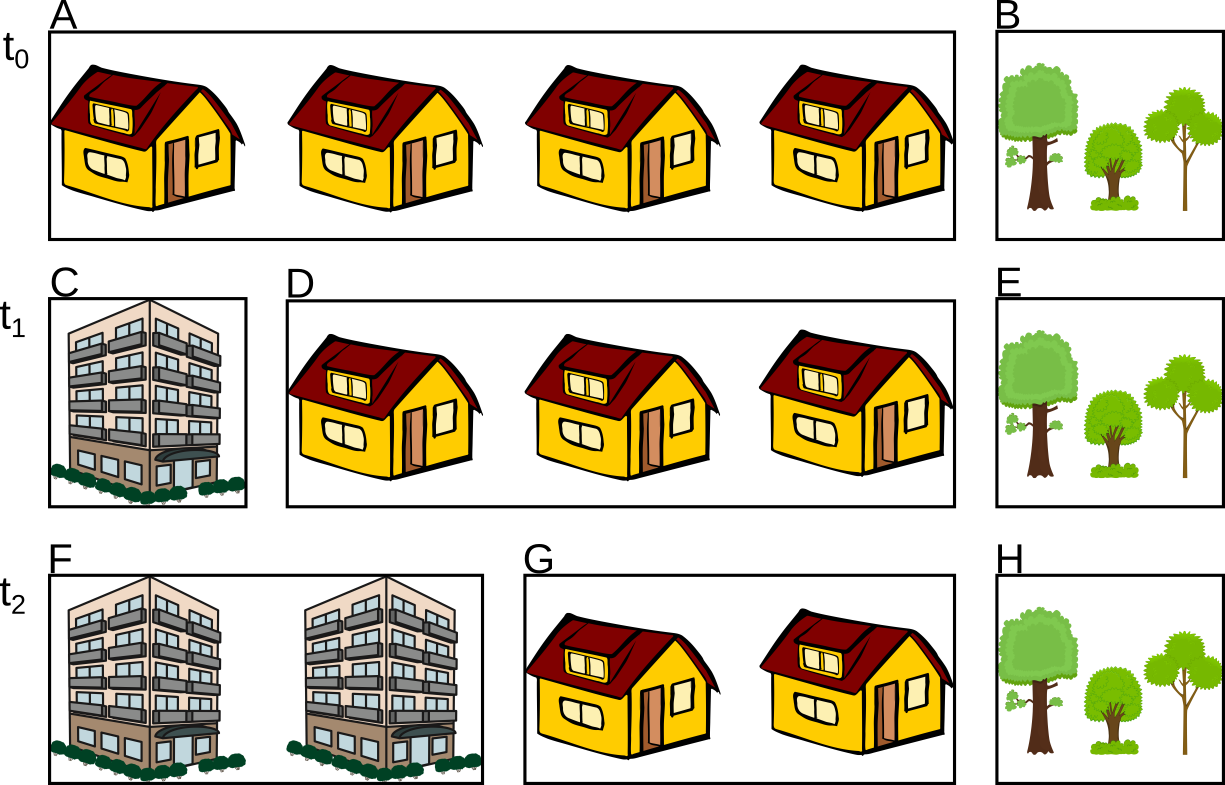
\includegraphics[width=0.475\linewidth]{intuition.png}
    }
    \subfloat{
        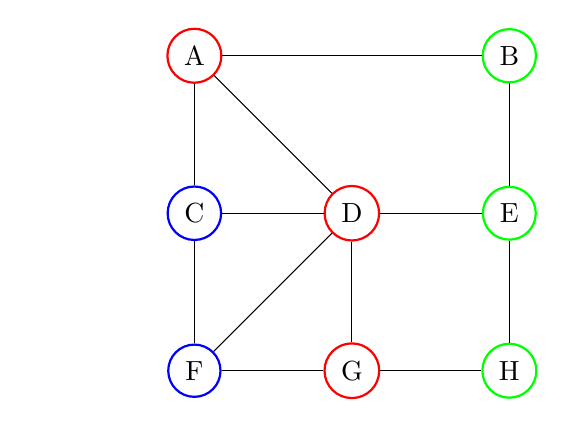
\begin{tikzpicture}
            \node (push) at (-2,0) {};
            \node [circle, draw=red, thick] (a) at (0,4) {A};
            \node [circle, draw=green, thick] (b) at (4,4) {B};
            \node [circle, draw=blue,  thick] (c) at (0,2) {C};
            \node [circle, draw=red, thick] (d) at (2,2) {D};
            \node [circle, draw=green, thick] (e) at (4,2) {E};
            \node [circle, draw=blue, thick] (f) at (0,0) {F};
            \node [circle, draw=red, thick] (g) at (2,0) {G};
            \node [circle, draw=green, thick] (h) at (4,0) {H};
            \draw (a) -- (c);
            \draw (a) -- (b);
            \draw (a) -- (d);
            \draw (b) -- (e);
            \draw (c) -- (f);
            \draw (c) -- (d);
            \draw (d) -- (f);
            \draw (d) -- (e);
            \draw (d) -- (g);
            \draw (e) -- (h);
            \draw (f) -- (g);
            \draw (g) -- (h);
        \end{tikzpicture}
    } \caption{Network based spatio-temporal data representation. \textbf{Left}:
    Three temporal stages of the evolution of a fictitious urban area, with
    aggregation areas A to H. \textbf{Right}: Network representation of the
    aggregation areas where the colours identify similar regions.
        \label{fig:intuition}}
\end{figure}

Instead, we propose a network-based representation. A \emph{network} (also
called a \emph{graph}) is a collection of entities (nodes) that are related to
each other (edges). In this case, each different aggregation area is represented
as a node and we connect nodes that have overlapping geographical areas\revision{ in
different times or are neighbours in the same time}, leading to the network
illustrated on the right of Figure~\ref{fig:intuition}. By partitioning the
network into connected nodes that are similar, we are effectively identifying
clusters in the spatio-temporal data, as illustrated by the colours of the nodes
on the right side of Figure~\ref{fig:intuition}. Further, all the possible paths
of change can be obtained by computing sequences of nodes over time, in this
case: (A, C, F), (A, D, F), (A, D, G), and (B, E, H). This representation is
also suited for geographically consistent regions, as illustrated by the stable
park in this example, and is therefore a generalisation of the traditional
paradigm.

%I'm adding this because Jeff Allen (Farber's guy) struggled with this.
Note that the edges of this network merely encode that two regions are related.
This is binary information, there is no apportionment, no areal measurements,
no population percentages associated with the edge. Indeed, our method also
connects regions of the same time that share borders, representing exactly that
they are neighbouring areas.

In the following, we argue that this network representation allows us to study
neighbourhood change in a way that does not require an prior interpolation. 


\section{Related Work}
\label{sec:related}

Since our problem encompasses several fields, we divide this section into
specific sub problems: \emph{longitudinal demographic studies}, describing the
traditional tabular approach to longitudinal studies; \emph{data
representation}, elaborating how evolving geographic data can be represented for
processing; \emph{data clustering}, briefly reviewing existing clustering
methods; and \emph{cluster characterisation}, articulating how clusters can be
visually summarised.

\subsection{Longitudinal demographic studies}
Census data is used not only to discover demographic
patterns~\citep{Firebaugh2016}, but to correlate demographic characteristics to
other measurements~\citep{diez1997neighborhood}. However, longitudinal studies
are rare, because they are difficult : \emph{"(...) One of the most challenging
and fascinating areas in spatial statistics is the synthesis of spatial data
collected at different spatial scales(...)"}~\citep{gotway2002combining}. While
census tract level data is readily available for the US since at least
1910~\citep{nhgis}, most studies consider the period between 1970 and 2010,
using pre-harmonised data from the Longitudinal Tract Data
Base~\citep{Logan2014}. Despite its inherent
errors~\citep{Logan2016,Hallisey2017}, this dataset has become the standard
source for longitudinal demographic data at the neighbourhood scale, with
similar efforts appearing in other countries~\citep{Liu2015,Lee2015,Allen2018}.
These datasets have been highly significant for the field. Yet they also limit
the universe of  data that can be used to study neighbourhood change, since any
new datasets would need to be similarly processed in order to be rendered
compatible with these sources. 

Another option considers the use of grid
data~\citep{Dmowska2017,Dmowska2018,stepinski2019imperfect}. Beyond the
increased spatial accuracy, this approach does not require complex harmonisation
when new data is considered, if the grids are compatible. However, demographic
data is usually not available in this format, especially from older sources.
Additionally, the conversion from tabulation areas can introduce significant
errors.

Given these challenges, it is worth considering new alternatives. In this work,
we propose a novel methodology that entirely avoids the problems of geographical
harmonisation, considering each measurement using its actual geographic region.
It does not require regions to be consistent across time because they are
naturally represented as different entities. 

\subsection{Data representation}

Network based representation of geographic information is fairly well explored
in the literature, as a basis for topological methods for event
detection~\citep{Doraiswamy2014}, leveraging signal processing on
graphs~\citep{shuman2013emerging,sandryhaila2013discrete} to find patterns and
outliers~\citep{Valdivia2015,Dias2015,Alce2018}. Networks are well suited to
represent trajectories as
well~\citep{VonLandesberger2016,Huang2016,chen2015survey}, allowing the use of
graph visualisation methods~\citep{Vehlow2015,Beck2014}. Our proposed method
builds upon this literature. We leverage a network-based representation that
removes the requirement for consistency in the measurement regions. Each region
in time corresponds to a different node. Instead of a collection of time-series,
the data is represented as a dynamic network. 

Networks have been used to represent census data for clustering purposes
~\citep{Dias2015,Setiadi2017}, but these works did not explore temporal
evolution, where they are particularly powerful. Networks allow a natural
representation of these inconsistent regions, with both spatial and temporal
connections. There are other possible representations that have similar
properties, but we adopted networks to allow the use of the vast existing
literature and methods.


\subsection{Data clustering}

Data clustering is one of the elementary processes for data analysis,
simplifying the data into a smaller number of homogeneous sets that can be
interpreted in the same way. There is no shortage of contributions for this
problem~\citep{Fahad2014}, but most neighbourhood related applications still
rely on k-means~\citep{jain2010data,Delmelle2016} and, to a lesser extent, Self
Organising Maps~\citep{Delmelle2017,Ling2016}.

However, a method for geographic data analysis should not ignore the geographic
component of the data, and we extend research exploring ways to incorporate it.
One straightforward option for agglomerative methods~\citep{han2001spatial} is
to consider only nearby clusters for merging~\citep{Chavent2017}, which can also
be done for k-means~\citep{soor2018extending}. Alternatively, the spatial
distance could be directly added to the inter-cluster metric~\citep{Chavent2017}
via a mixing parameter, which adds flexibility to the method, but introduces the
problem of finding the correct application-dependent values.

Indeed, one crucial step in most clustering algorithms is the definition of the
number of clusters. We avoid this problem by considering hierarchical
methods~\citep{soille2012morphological}, where the result is not a partition of
the data, but a tree of partitions, similar to a dendogram. This approach is
interesting for interactive methods, because it allows the user to change the
number of clusters on the fly. Since our data is represented as a network, we
opted for an heuristic variation of the maximum weighted matching algorithm
called \emph{sorted maximal matching}~\citep{markus2017}, which merges clusters
based on the weights of the edges between pairs of clusters. 



\subsection{Cluster characterisation}
While visualisation has gained prominence as a crucial component of scientific
discovery, justification, and communication \todo{Add Cites: maybe Gelman?
Tufte?}, visually representing evolving spatial data is a challenging old
problem~\citep{monmonier1990strategies,andrienko2003exploratory,ferreira2015visual,Zheng2016}.

Most geographic data is naturally bidimensional and maps work well in this
case~\citep{Zheng2016,ward2015interactive}, but the additional temporal
dimension cannot be so naturally represented. One straightforward option is to
leverage tridimensional plots~\citep{andrienko2014visualization,Tominski2012a},
but this can lead to visual obstructions or scaling problems unless a
tridimensional display device is used. A simpler, well adopted,
option is to display a map that corresponds to a subset of the temporal
information, allowing the user to change the time with an associated
control~\citep{Chen2017,Valdivia2015,Alce2018,Doraiswamy2014}. Small multiples
can be used~\citep{VonLandesberger2016}, but only when there are few temporal
snapshots. However, none of these options is suitable to represent many
variables at the same time.


Using data clustering, we can represent the region's cluster instead of all the
its variables~\citep{Alce2018,Valdivia2015,VonLandesberger2016}. While this
simplifies the geographic portion of the visualization, it introduces the
problem of how to summarise the contents of each cluster. One traditional
approach is to use parallel coordinates plot~\citep{ferreira2015urbane}, but
these they can get cluttered representing similar clusters over several
variables. Further, for demographic applications, the clusters are usually
strongly characterised by a small subset of
values~\citep{Delmelle2016,Delmelle2017}. Therefore, in the proposed method, we
identify the variables that are most relevant to the characterisation of each
cluster. The distribution of values on that variable is then represented using a
boxplot, a well known statistical plot displaying basic properties of the
distributions.

% \section{Design considerations}
The development of our tool was guided by experts in urban sciences and
sociology whose main concern is to identify similar groups and how they evolved
over time, with as much detail as possible.


Practically, beyond the basis requirement that our method needs to be able to
work with non-geographically harmonized data, we divided the other requirements
into two different categories: \textit{Method}, the practical aspects of the
clustering method and classification, and \textit{Interface}, concerning the
visual representation of the information.

\begin{enumerate}
    \item[M1]{\textbf{Geographical information}: The clustering method needs to
    consider the available geographical information along with the data
    associated to the region.}

    \item[M2]{\textbf{Parameter configuration}: The configuration parameters for
    the clustering method should be configurable by the user.}

    \item[I1]{\textbf{Temporal evolution}: The evolution of each region over
    time can be inferred by its associated clusters. This evolution needs to be
    easily represented. }

    \item[I2]{\textbf{Cluster characteristics}:  The visual representation of
    each cluster should easily convey its relevant characteristics, including
    both geographic and content information.}

    \item[I3]{\textbf{Details of the changes}: Once a geographic region is
    selected, the interface should clearly convey how the associated information
    changed over time.}
\end{enumerate}


\section{Visualising the demographic spatio-temporal evolution}
\label{sec:method}
Figure~\ref{fig:overview} presents an overview of the processing steps of the
proposed method, illustrating how the nodes of the network are used to represent
the regions. The following sections elaborate this figure and explain the main
features of the interface we built to visualise and explore the evolution of
neighbourhoods on the basis of our proposed method.


\begin{figure}
    \centering 
    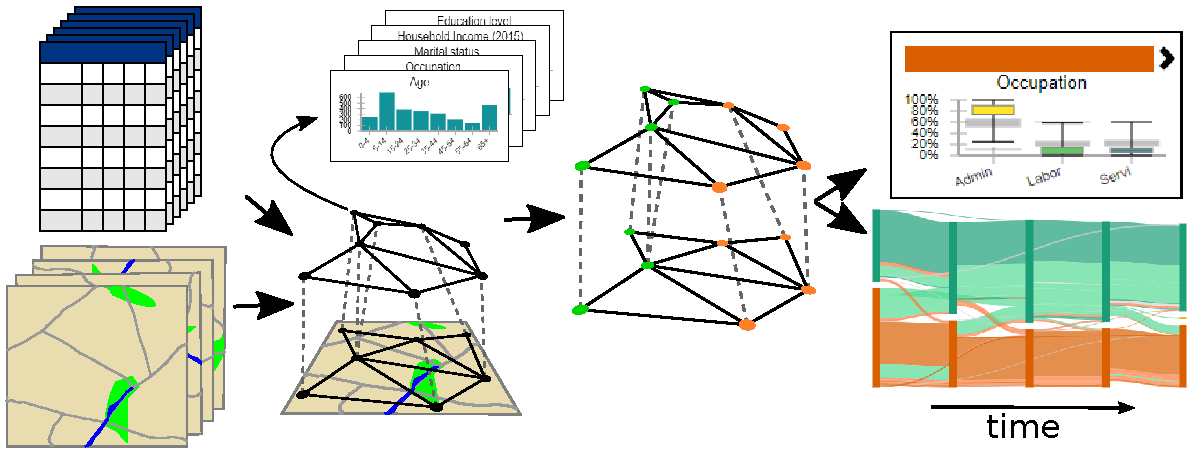
\includegraphics[width=0.975\linewidth]{overview.pdf}
    \caption{Overview of the proposed method. A network is generated combining the
        original census data, encoding the changing geographical information.
        The network is partitioned into an hierarchy~\citep{markus2017}. The
        characteristics and evolution of the clusters are then visually
        represented.
        \label{fig:overview}}
\end{figure}


\subsection{Census methodology and data representation}

Census data is disseminated in a tabulated form for aggregation areas: whole
country, state/province, metropolitan region, and so on. To allow for a more
meaningful comparison of the data, we aggregated related variables (e.g. White,
Black, Asian, Other) into what we called an \emph{aspect} (e.g. Race). The
aspects are represented using normalised histograms. This normalisation is
crucial for direct comparison. In essence, it is a generalisation of the
standard method of comparing percentages, since each aggregation area has a
different total population.

Each area of each census year is represented as a node, and edges are placed
between nodes if the corresponding regions share geographic borders in the same
year. Further, edges are placed between nodes if the corresponding regions
belong to sequential years and \revision{their geometries intersect. To avoid
spurious connections caused by geometry fluctuations, one of the geometries is
slightly shrunk before the intersection, using a buffer of -1e6. More
importantly, while weights will be associated with these edges before they are
processed, they are not derived from the geometry, but from the data. The actual
intersection area is not considered in this representation. } This approach
leads to a single network representing the whole spatio-temporal space of the
data. Our objective then becomes to identify partitions of this network such
that the nodes of each partition are more similar between themselves than to the
other nodes. 


\subsection{Geographic content clustering}
Having tied the regions together into a network, we can now partition it to
identify similar sets of regions. We start by adopting a distance function
between the nodes, measuring the difference between the data of the regions.
This value is then associated with the edges, leading to a weighted dynamic
network. Every node has a collection of histograms, each representing the
distribution of certain aspect in the population.

Let $\G=(\V,\E)$ be a network, where
$\V=\{\vertice_1,\vertice_2,\dots,\vertice_n\}$ is the set of nodes and
$\E=\{(\vertice_i,\vertice_j), i\not=j\text{ and }i,j \in [1,n]\}$ is the set of
edges. A function $\Hist$ associates each node to a set of $K$ histograms. We
define the distance $\D$ between two nodes $\vertice_i$ and $\vertice_j$ as:

\begin{equation}
    \D(\vertice_i,\vertice_j)=\sum_{k \in [1,K]}{\weight_k\, d(\Hist_k(\vertice_i),\Hist_k(\vertice_j))}
    \label{eq:dist}
\end{equation}

\noindent where $d$ is a distance metric between histograms and $\weight$ is a
sequence of non-negative weights associated with each aspect,
$\sum_{k\in[1,K]}{\weight_k}=1$. While any histogram metric can be used, we
adopted a euclidean distance between the vectors, because it led to reasonable
results with reduced computational cost. Therefore the distance between two
nodes is defined as the weighted average distance between its associated
histograms, where the weights can be adjusted by the user.

Once the distances are associated to the edges, we use watershed
cuts~\citep{Cousty2009} to create an initial clustering, which is then refined
into a hierarchy using the Sorted Maximal Matching (SMM)~\citep{markus2017} with
median linkage. The initial watershed step is performed to create an initial
clustering and reduce the running time of the SMM. We introduced one new
parameter to this method: a maximum distance threshold for the merges, to avoid
the early merging of outliers. We refer the reader to the original
paper~\citep{markus2017} for more details, including a complete performance
evaluation using several metrics. \revision{We chose this algorithm because it
is simple and easily customisable, and while different algorithms will lead to
different results, our methodology should work with any hierarchical clustering
algorithm.}


Each resulting cluster is contiguous in the network. This means that two
similar, but non-contiguous, sets of areas will be classified into two different
clusters, which can be counter-intuitive. To overcome this issue, we
\emph{augment} the network with two new edges per node from a nearest neighbours
graph~\citep{scikit-learn} using only the distances between the histograms.
These edges connect nodes with similar content, if they are not already
connected, providing a path for the algorithm to group similar nodes.
\revision{The regions connected by those edges will be merged on the first
stages of the clustering, since they are very similar, leaving the remaining
steps of the hierarchy to be determined only by the geographical edges. We
explored with different numbers of augmentation edges, but the results were not
consistent, since the distribution of the edges is data dependent. Adding two
edges per node was the least number of edges that led to stable and consistent
results in the scenarios available in our prototype. Since the problem of
balancing the data space with the geographical space is relevant for
geographical data analysis, this methodology potentially warrants further
exploration, beyond the scope of this work.}


\subsection{Cluster characterisation and variable relevance}
\label{sec:relevance}
A crucial step in understanding neighbourhood change is to characterise the
evolving clusters.  The composition of each cluster is represented here by
simple statistical measures, considering each aspect separately. We compute the
minimum, maximum, median, 25\%, and 75\% quantiles for each variable of each
aspect for all clusters in the hierarchy. While interpreting these values is
more complex than interpreting just the average, they provide far more
information about the underlying distribution.


We also use these statistical measurements to discover what characterises each
cluster, that is, what makes it different from the others.  We define the
\emph{relevance} of a variable of an aspect based on the distance between the
interquartile ranges (IQR) of the clusters in the same hierarchical level. If
the IQRs overlap for all clusters, that variable is not relevant to the
characterisation of the cluster, but if the IQRs are distant, it means that this
specific range of values is something that only occurs in this cluster.
Examining IQRs therefore provides users a straightforward visual method for
determining what variables most clearly define a given cluster.


\subsection{Clusters and trajectories}
While the partition of the data into different clusters helps the user to
understand what groups exist and where they are, we are also interested in the
evolution of these groups. To examine this process of evolution directly, we
introduce the concepts\revision{of \emph{temporal paths} and \emph{trajectories}. 

We call a temporal path any sequence of nodes in our representation network such
that the temporal information associated with the nodes only increases. For
instance, in Figure~\ref{fig:intuition}, the sequences ACF, ADF, ADG, and BEH
are temporal paths. With harmonised data, the time-series of to each region
would form a temporal path, each node would be connected only to its older and
newer versions, belonging to only one temporal path, as illustrated by the path
BEF. Since our data is not harmonised, more connections are allowed and each
node can belong to an arbitrary number of paths.

Semantically, this is a generalisation of the idea of geographical time-series,
because each temporal path is one possible option for the data to change over
time. Returning to Figure~\ref{fig:intuition}, the paths ACF, ADF, and ADG all
start on the same homogeneous region, but evolve differently over time. In other
words, this network encodes the information that portions of the region A
changed to form regions C and D, but we do not know specifically which parts,
nor we need to, since the same region can belong to several temporal paths.
Interestingly, when interpreted in this framework, geographical harmonisation is
a method to split and/or merge nodes so each belongs to a single temporal path.

Since each node in the sequence that forms the temporal paths has an associated
cluster, we can classify the paths based on the sequence of clusters. We call
each unique sequence of clusters present in this result a \emph{trajectory}.
Regions on the same trajectory had the same sequence of clusters, therefore had
similar temporal evolution.}

\subsection{User interface}
\label{sec:ui}
To validate and explore the results of our methodology, we built a user
interface, illustrated in Figure~\ref{fig:ui}, considering census tract (CT)
level data from the Chicago region between 1970 and 2010. This region is known
for its entrenched racial divide and the emergence of a \emph{'young urban'}
population with a higher education level~\citep{Delmelle2016,Delmelle2017}. More
details are presented in Section~\ref{sec:study}.


\begin{figure*}
    \centering 
    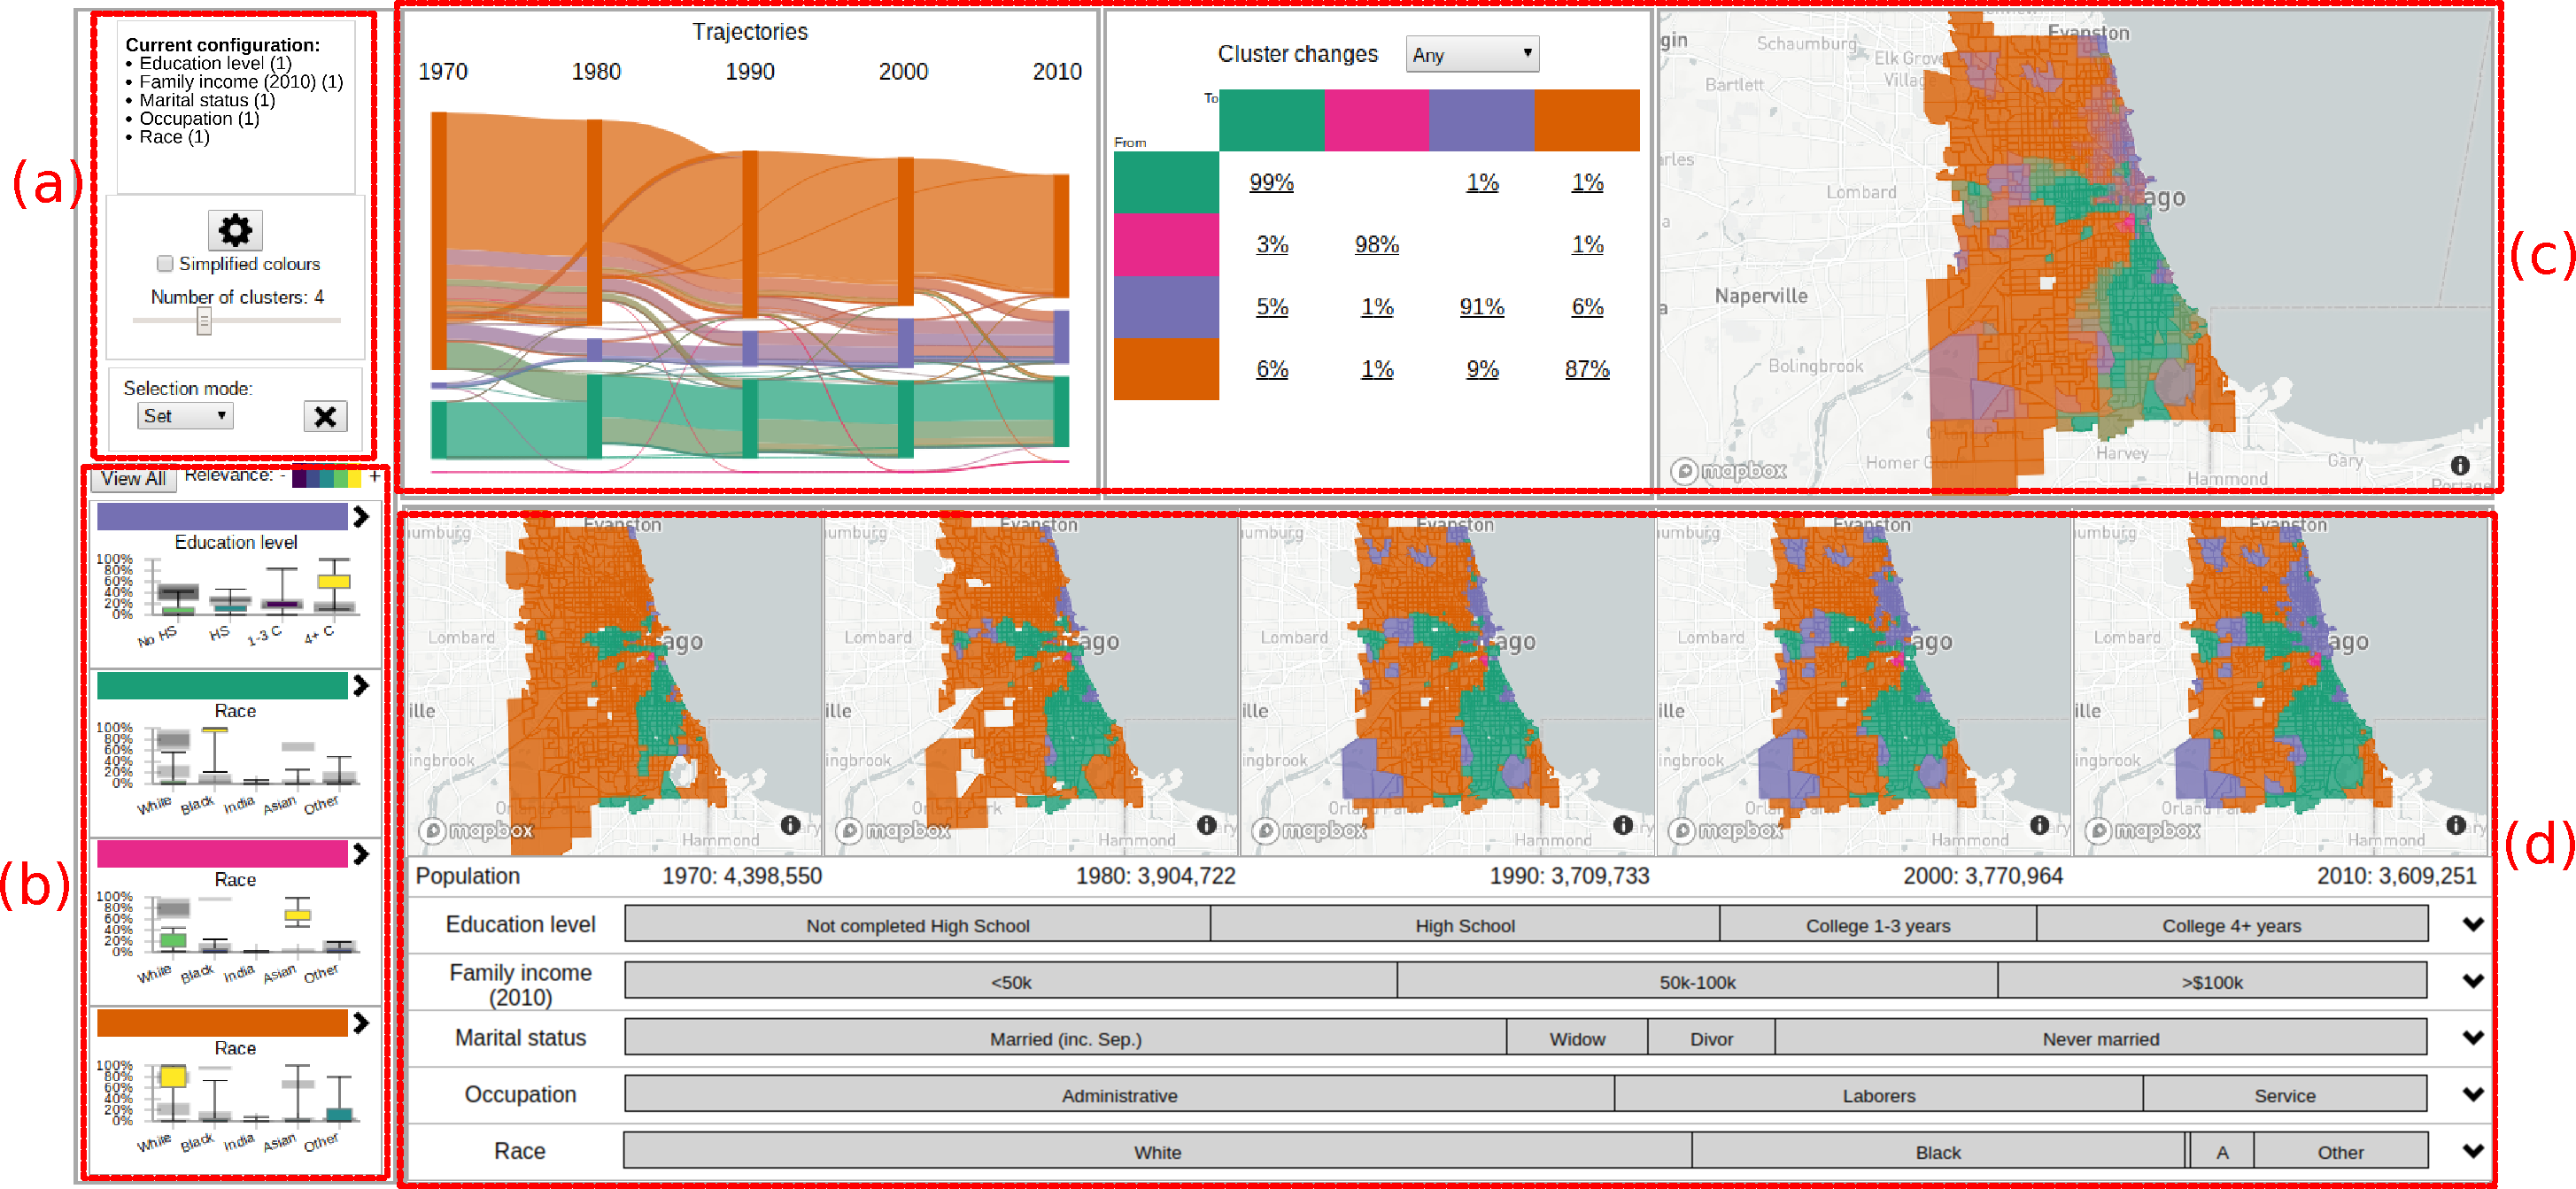
\includegraphics[width=0.975\linewidth]{ui.pdf}
    \caption{Initial interface of our method showing the demographic evolution of Chicago. 
        \textbf{(a)}: Configuration panel with the current clustering parameters and controls.
        \textbf{(b)}: Cluster overview illustrating the most relevant aspect for each cluster. 
        \textbf{(c)}: Trajectories overview and the general evolution of the population, geographical information, and how it changed. 
        \textbf{(d)}: Details of the selected trajectories, including precise geographic locations, population numbers, and the composition of the aspects.\label{fig:ui}}
\end{figure*}


As illustrated by Figure~\ref{fig:ui}, our proposed interface heavily relies on
colour to express cluster-related information. We adopted this convention
because colours can be used in all our visual tools in a coherent manner.
However, there is a limit on the number of distinct colours that can be used. We
limited the number of clusters to eight because this was the largest number of
colours that we could reliably and accessibly use, derived from the 8-class
Dark2 set from ColorBrewer~\citep{ColorBrewer}. 


The configuration panel, on top left in Figure~\ref{fig:ui}, displays which
aspects were used and their weights (following Equation~\ref{eq:dist}). It also
includes other configuration options that can be altered without re-processing
the data, such as the number of clusters and the colour option. The gear button
allows access to the other configuration options that do require further
processing, such as changing location, aspects, and weights. 


The cluster overview panel, on the bottom left in Figure~\ref{fig:ui}, displays
a brief summary of each cluster, based on the distance between the IQRs, as
detailed in Section~\ref{sec:relevance}. The \emph{View all} button opens a new
panel where all aspects are included, while the chevron at the side lets the
user expand each cluster separately. 

We adopted an \emph{enhanced} version of the traditional boxplot, which includes
the IQRs for the other clusters, in slightly larger and faded black rectangles.
We also colour the current IQR according to its relevance.  For instance, the
boxplot that summarises the purple cluster illustrated in Figure~\ref{fig:ui},
detailed on Figure~\ref{fig:boxplot}, illustrates that this cluster is best
defined by the proportion of the population with four or more years of college.
The user can quickly see that this is relevant because the corresponding IQR is
coloured with the highest relevance present in the legend. It is also clear
that, while this cluster includes CTs that have between 10\% to 90\% of people
in this variable, approximately, half of them have about 60\% of the population
with four or more years of college. Since all the other IQRs are well separated,
this is a defining characteristic of this cluster. Conversely, the proportion of
the population with one to three years of college is not relevant, as indicated
by black fill in the rectangle representing the IQR of this cluster, in
overlapping position with the rectangles of the other clusters. By clicking on
the coloured bar above the boxplot, the user can select all trajectories that
contain this cluster at any point in time.

\begin{figure}
    \centering 
    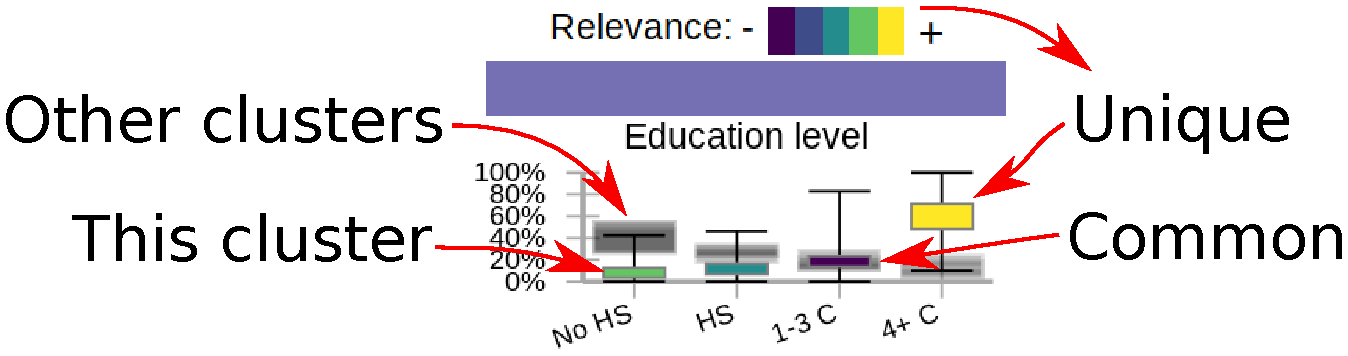
\includegraphics[width=0.45\linewidth]{boxplot.pdf}
    \caption{Enhanced boxplot of the clusters' characteristics allows a quick
    comparison to the other clusters.\label{fig:boxplot}}
\end{figure}


The trajectories overview aims to convey basic information about the
trajectories, where they are, and what changes are involved. This is done using
three sub panels. The first, on the left, contains a Sankey diagram illustrating
the evolution of the clusters over time. The widths are proportional to the
population involved. In our example in Figure~\ref{fig:ui}, the orange and green
clusters contain most of the population and are fairly stable over time. The
pink cluster is small and mostly stable. The purple cluster is increasing,
mostly by incorporating areas that were previously orange. Since the purple
group corresponds to the emergent 'young urban' group, this corroborates the
findings of Delmelle~\citep{Delmelle2016,Delmelle2017}, showing that our
network-based method can recover results from the traditional data processing
approach.

In the next panel, illustrated in the top middle of Figure~\ref{fig:ui}, is a
transition matrix between the clusters. It indicates a rounded percentage of the
population whose area changed between each pair of clusters. This kind of table
can be found in the related literature~\citep{Delmelle2016}, so it is familiar
to the advanced users. It not only informs the proportional changes, but allows
the selection of the corresponding trajectories for further analysis.

The panel in the top right of Figure~\ref{fig:ui} is a map of the region under
analysis, summarising the geographical evolution of the clusters over time.  The
colours are derived from the clusters involved in each trajectory, which are
consistent across the linked views. 

The bottom part of the interface contains the details for the selected
trajectories, or for the whole city if nothing is selected, as illustrated in
Figure~\ref{fig:ui}. This panel contains two main regions: the small multiple
maps, depicting the clusters at each year, and the stacked bar plots that
summarise the overall composition of these regions. In this example, the maps
show the transition from orange to green and purple in several regions over
time. Clicking on a region in these maps will bring up a new panel with the
original census data of this specific region. The actual population numbers are
below the maps.

Each aspect is represented by a stacked bar plot, where the width of each
rectangle corresponds to the average percentage of that variable over the
considered period. In this case, about half of the people in Chicago in the
considered period are married, and the percentage that are Widowers or Divorced
is roughly similar. About half of the population work in Administrative jobs, a
third never completed high-school, approximately half have gross family income
below 50,000USD per year. The vast majority identify as white. Placing the mouse
over one of the bars will open a small panel with the temporal evolution of that
specific variable, and clicking on the chevron on the right side expands the
corresponding aspect, showing details of the temporal evolution of each variable
and also the corresponding IQRs for the whole city.

\section{Illustrative scenarios}
\label{sec:study}

In this section we present two illustrative scenarios, using census data from
the United States~\citep{nhgis} and
Canada\footnote{\url{http://datacentre.chass.utoronto.ca/census/}}, tabulated by
CTs,  from 1970 to 2010. 

The prototype interface allows access to 41 regions, 29
in the US and 12 in Canada. New York City was split into its boroughs to avoid
memory crashes on the client browser due to the high number of CTs.  We used
five aspects for the USA: Education level, Family income, Marital status,
Occupation, and Race; and seven for Canada: Age, Education level, Home language,
Household Income, Marital status, Occupation, Place of birth, and Religion. 

While our method does not require geographic harmonisation, it requires matching
the variables over time. The supplementary material contains the details of
which census columns were used for each aspect. Income is slightly inaccurate,
even though we did correct for the official inflation. We grouped the original
ranges into three larger ranges, but they do not match precisely.

\unsure{CHECK}\revision{1.12.(1-5)}{These results are meant to demonstrate the
utility of the interface for understanding the evolutionary dynamics of urban
neighbourhoods. They also show the face validity of the results generated by our
novel network-based approach. However, the US data for 2010 is  not from the
decennial census, but from the ACS 2006-2010, compromising the temporal
stability of the data. Further, the regions selected do not correspond to any
pre-defined regions (metros, cities, census areas), but to somewhat arbitrary
regions defined around a location of interest, making direct comparisons harder.
Since  variable matching is a  manual process, we selected a minimal set of
aspects for each country, which are not necessarily similar to each other, or
similar to studies in the current literature. These factors would seriously
hinder any study using the existing methods, but our results were well-aligned
with several other studies, illustrating the robustness of our approach to
imperfect conditions. }

\subsection{Chicago}
Our first scenario examines Chicago, using an arbitrary region larger than the
administrative borders. Its demographic composition is well explored in the
literature, with reports of racial divide and
gentrification~\citep{Delmelle2016,Delmelle2017,Hwang2014}, so we expect our
results to contain stable regions where the Race aspect is relevant, and some
degree of population change, with increasing income and education levels. 


The initial state of the prototype is illustrated in Figure~\ref{fig:ui}. The
first step is to identify the compositions of each cluster from the boxplots, so
orange is associated with majority of White population, green with majority
Black, and purple with higher proportion of four years of college or more (high
education level). The expanded version of the boxplots for the purple cluster
shows a higher income level and majority of occupations in administrative jobs,
therefore the purple cluster identifies gentrified regions.


The trajectories plot illustrates the process of gentrification, also
illustrated in Figure~\ref{fig:chiWorkflow}, progressively absorbing regions
from the orange cluster (White). This corroborates results from the literature
reporting that Black neighbourhoods are less likely to
gentrify~\citep{Hwang2014}. The transition matrix provides more details, showing
that around one percent of all regions that became purple at any time
transitioned from the green cluster (Black population), while nine percent were
previouly associated with the orange cluster (White). Next, we select the region
that is gentrified in 2010, by clicking on the corresponding rectangle in the
trajectories plot, updating the information on the maps and the details portion
of the interface.

The corresponding regions are highlighted in the maps, where the spatial pattern
is clear, corresponding exactly to previous findings in the literature based
upon harmonisation~\citep{Hwang2014}. Further, we can also identify the regions
that gentrified earlier on the small maps that depict the involved regions over
time. Since the most relevant aspect is Education, specifically "Four or more
years of college", we can expand the details of this aspect, as illustrated in
the rightmost portion of Figure~\ref{fig:chiWorkflow}, which is increasing for
the whole city (grey band), but faster and to a higher level in this region
(black band).



\begin{figure*}
    \centering
 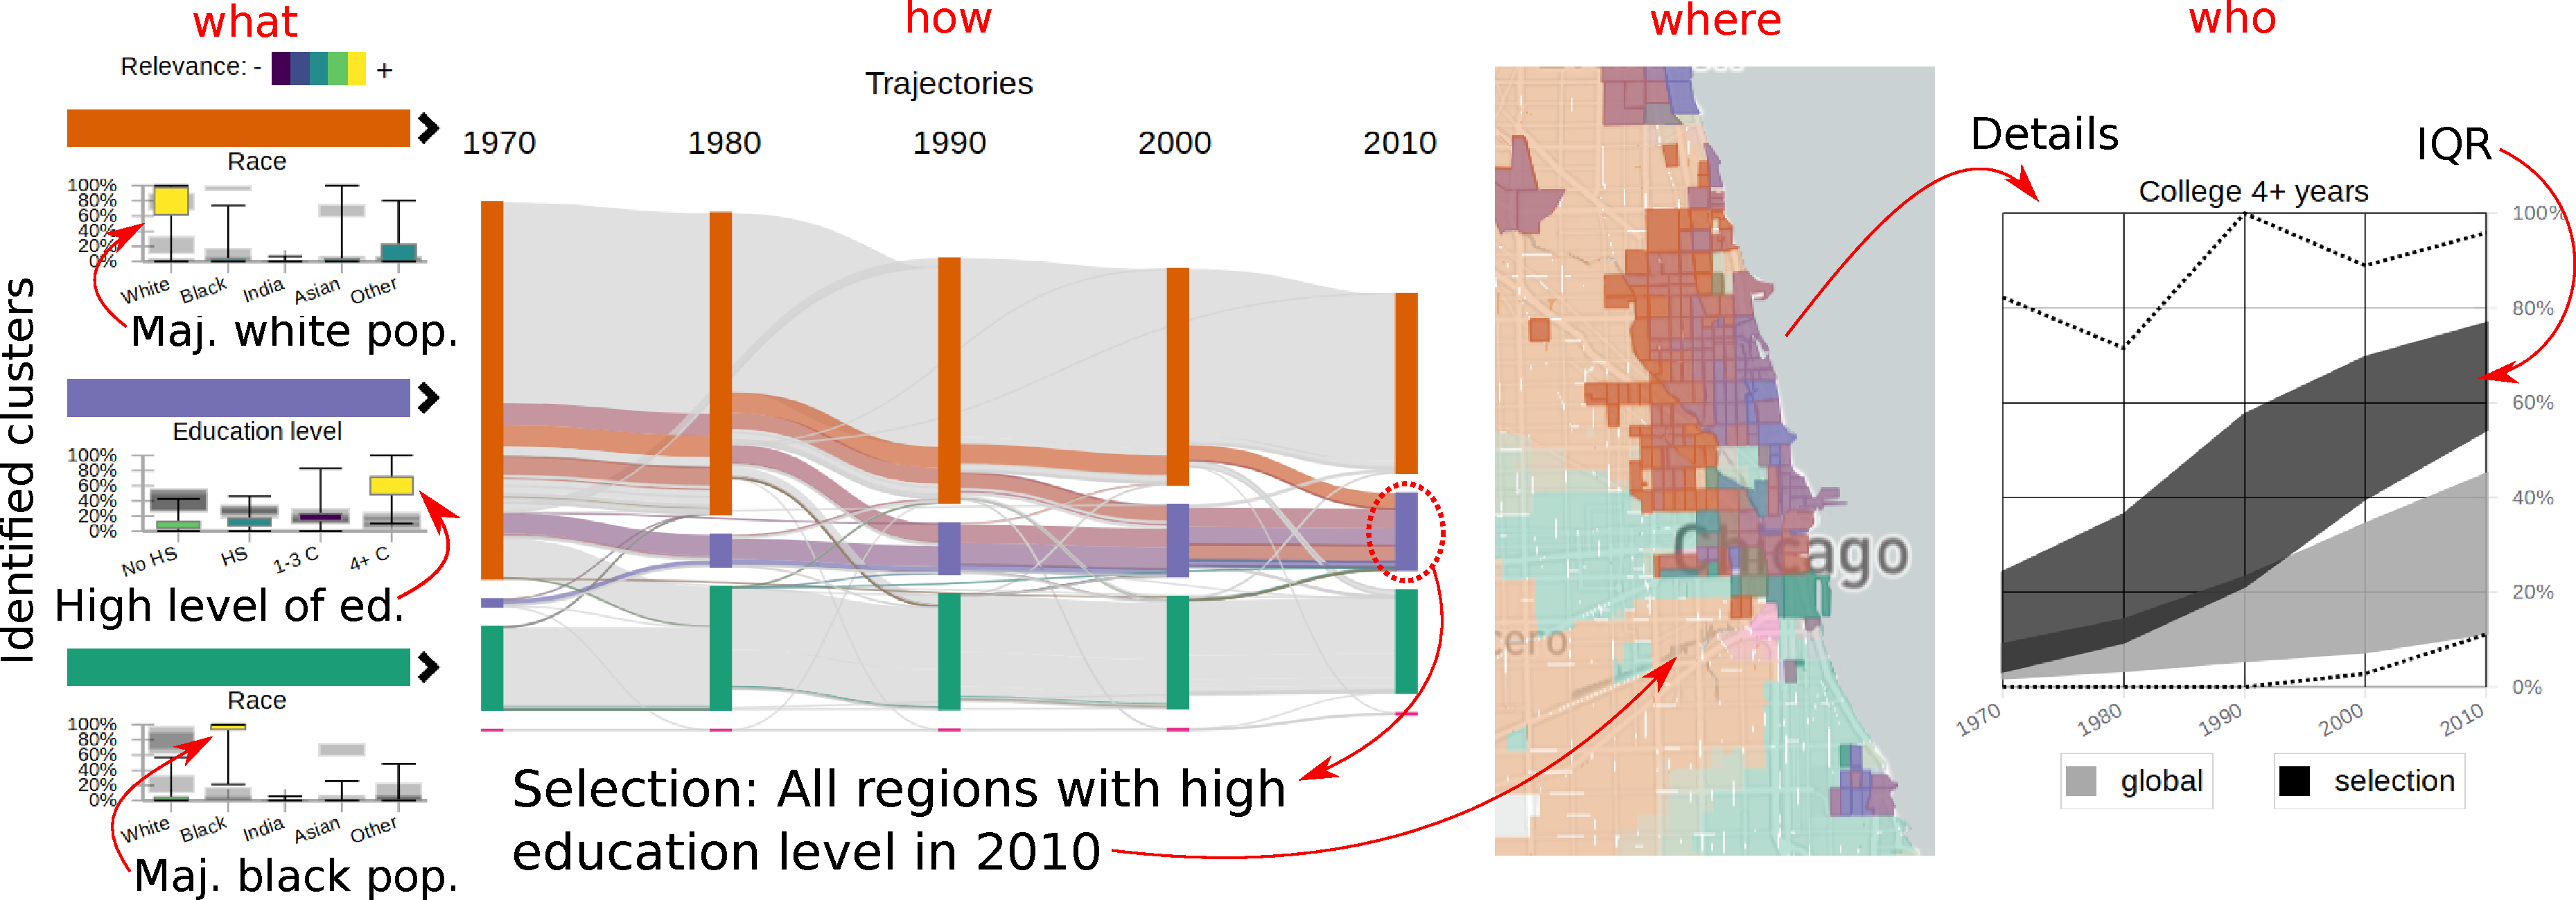
\includegraphics[width=0.9\linewidth]{newTeaser.pdf}
 \caption{Workflow to discover gentrification in Chicago: the purple cluster
 corresponds to high education / income. Its population is increasing over time,
 absorbing from the majority White cluster (orange). By selecting the purple
 cluster in 2010, the region is highlighted in the maps. The proportion of
 people with 4+ years of college is increasing in the whole city (grey IQRs),
 but significantly more in this region (black).\label{fig:chiWorkflow}}
\end{figure*}



\subsection{Toronto}

We consider a region that corresponds approximately to the administrative border
of the current city of Toronto, using all seven available aspects with equal
weights. While Chicago was fairly stable, Toronto is known to be a more dynamic
and diverse city, with significant and increasing immigrant
population~\citep{hulchanski2007three,Fong2011}, especially
Asian~\citep{Fong2003}. Toronto is also known for a stable and well defined
Jewish community~\citep{Harold2018, Fong2011}. Therefore, we expect \revision{1.14}{a}
combination of stable and dynamic regions on the results, with Place of Birth,
Home Language, and Religion identified as relevant aspects. The results are
summarised in Figure~\ref{fig:to}, considering eight clusters.

\begin{figure}
    \centering 
    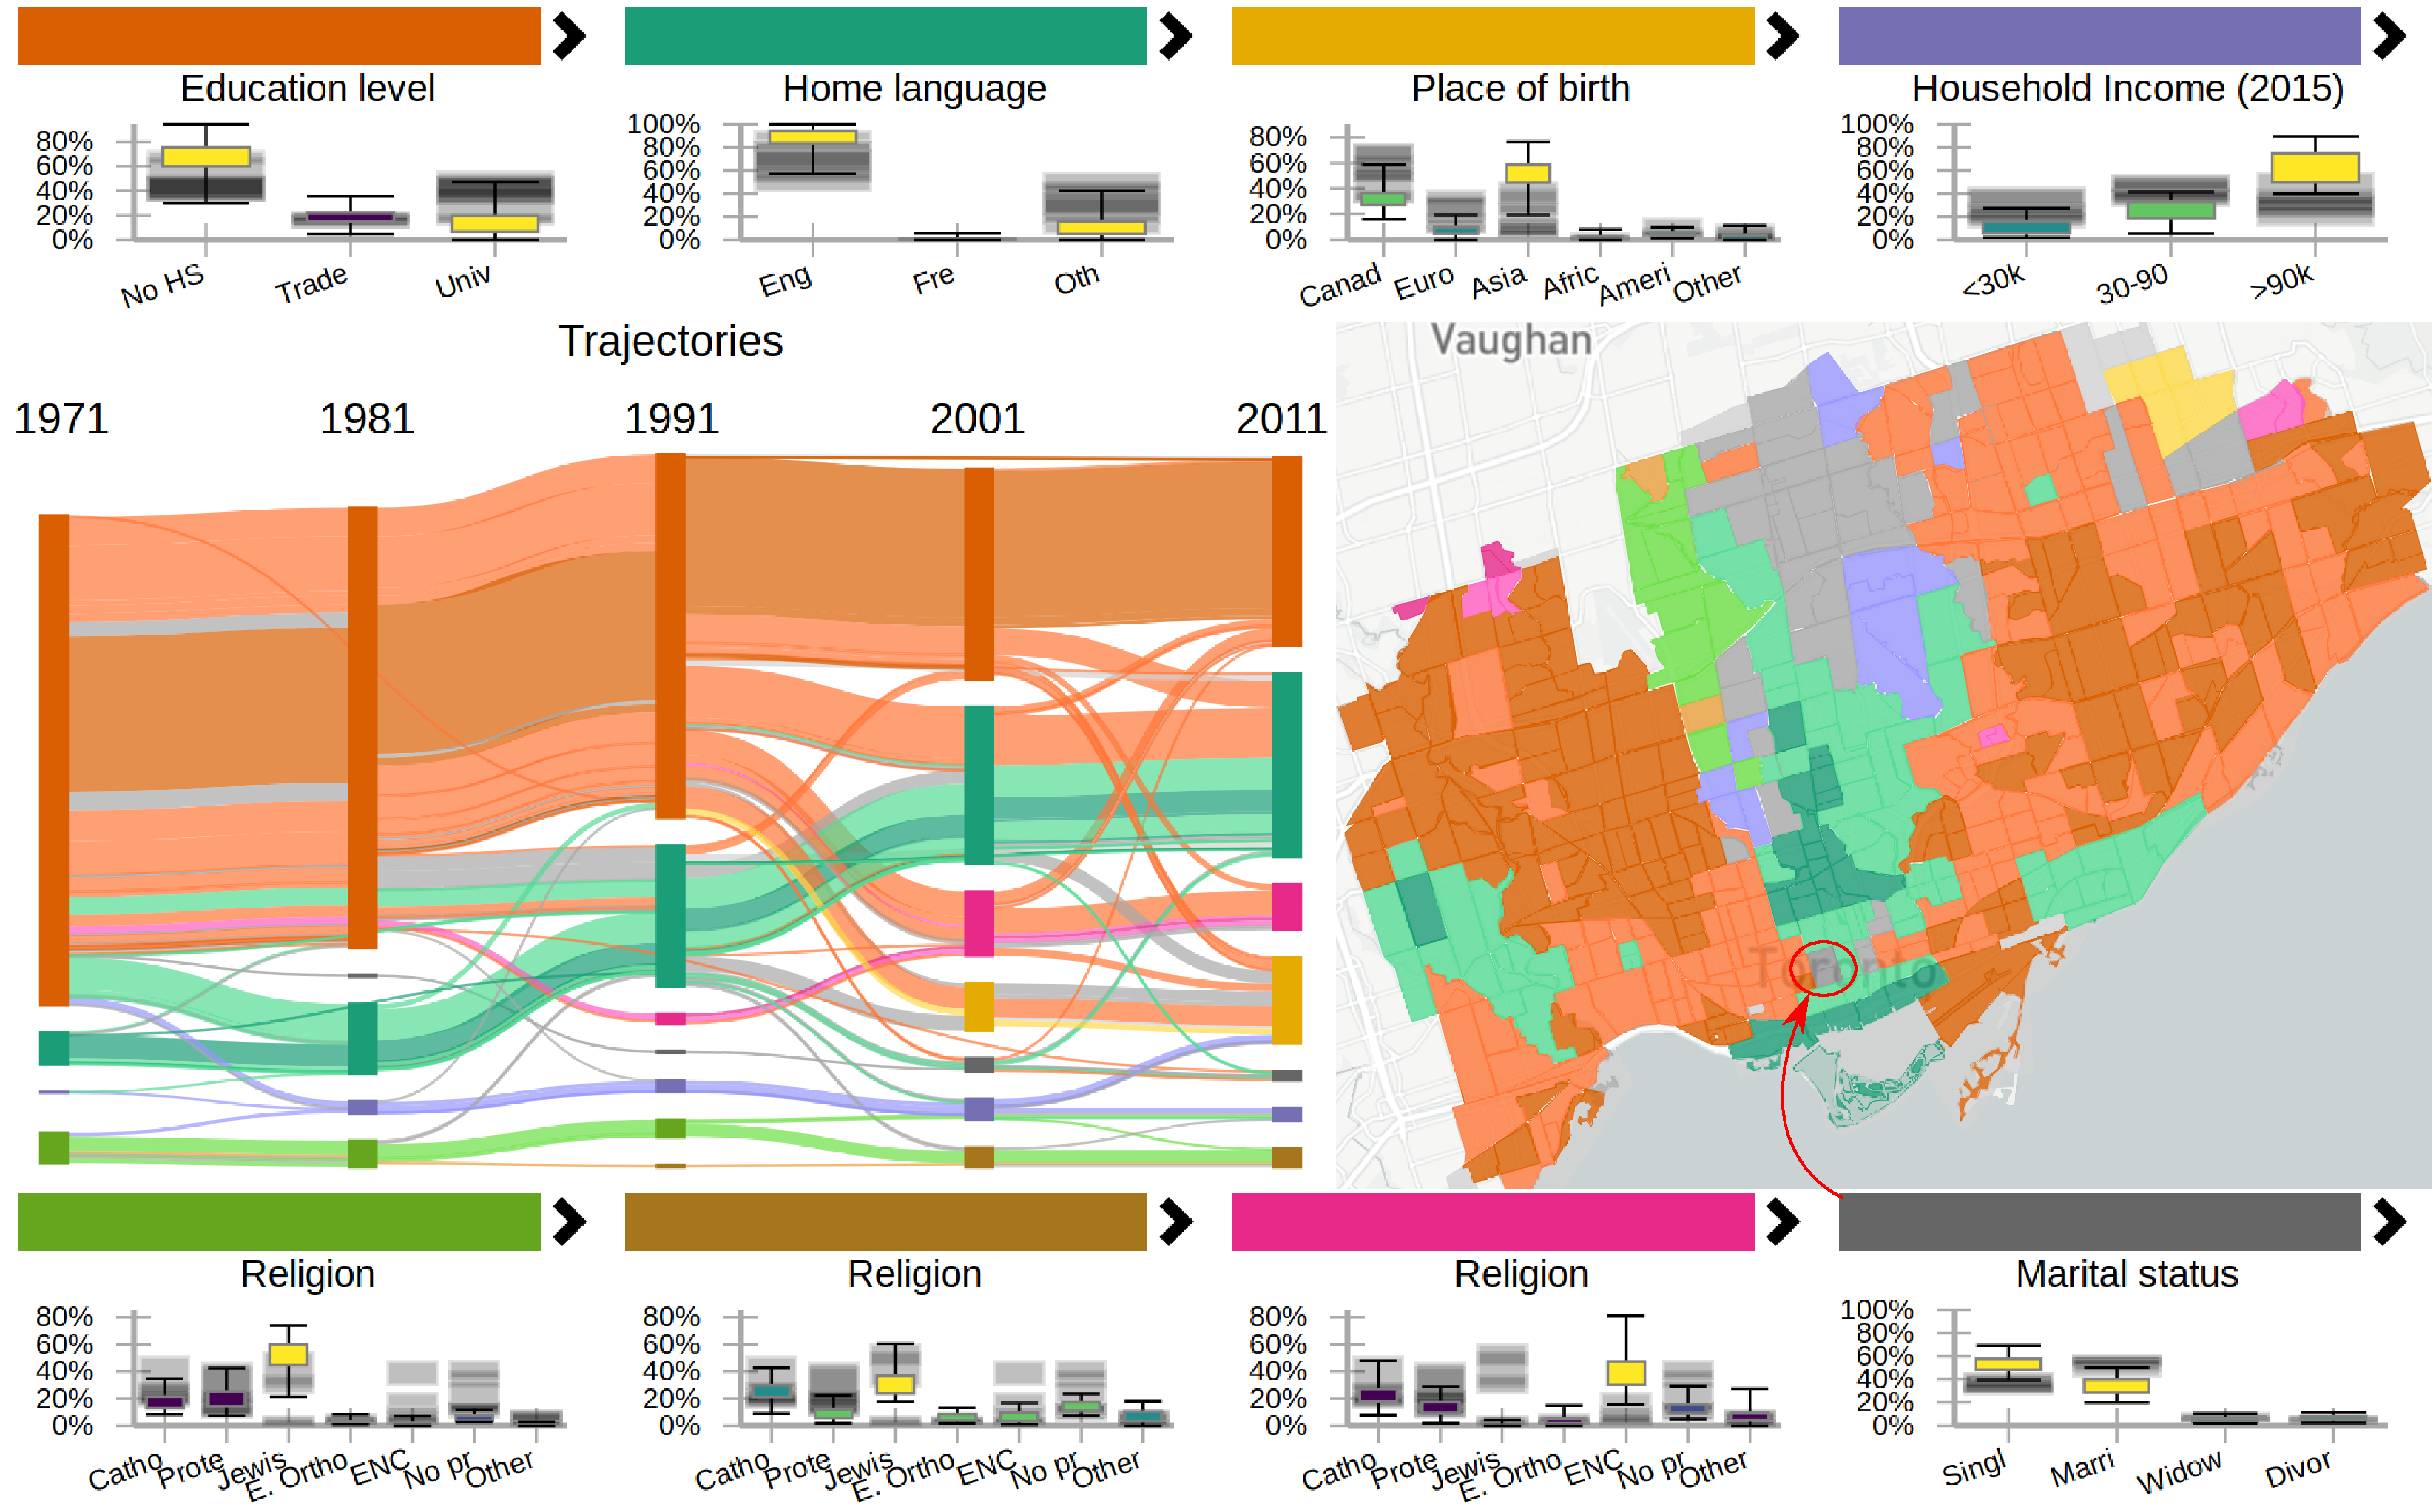
\includegraphics[width=0.85\linewidth]{to.pdf}
    \caption{Clustering results for Toronto, with eight clusters, including
    clusters representing Jewish population, high and low income, low education,
    and Asian immigration.\label{fig:to}}
\end{figure}

The population with low percentage of University degrees is represented in
orange, mostly anglophone population in green, Asian immigrants in yellow, high
percentage of income in the highest bracket in purple, high percentage of Jewish
people in light green and brown, high percentage of Eastern Non-Christian
religion in pink, and high concentration of single people in dark grey. From the
trajectories plot, we can see that Toronto is more dynamic than Chicago, with
one cluster constantly shrinking. In the 1970s, the city was divided into four
clusters: low number of university degrees, Jewish population, majority
anglophones, and high income. Interestingly, the more recent clusters that
absorbed regions from the orange cluster have similar education profiles and are
differentiated by other aspects. In this sense, the city is growing diverse,
changing from a common low education profile to a higher level of education with
more diversity in religion (pink) and immigration (yellow).


Indeed, the growing Asian population is visible starting in the 1980s and
building thereafter, leading to the yellow and pink clusters. While both include
a high percentage of people born in Asia, the pink is more defined by religion,
with low percentage of university degrees, and contains the lowest percentage of
people in the highest income bracket for these clusters; the yellow is less
defined by religion, and has higher education and income, geographically
corresponding to the Markham region, know for its Chinese population. A similar
division also happens for the two Jewish clusters, where the light green cluster
has lower education and income levels than the brown cluster. The purple cluster
of high income is somewhat stable. Until 2011 the cluster included the Bridle
Path neighbourhood, known for its wealthy population. In 2011 it was classified
into the yellow cluster of Asian immigration, since about 40\% of the population
for this CT were then born in Asia. The income distribution did not change, with
85\% of the population with an income of 90k CAD or more.


The most significant indicator of Toronto's dynamism is the presence of grey
regions on the map. These represent regions associated to three or more clusters
over this five census period. Using the 'Add' mode for the trajectory selection,
we select their trajectories, and a subset of the details is illustrated in
Figure~\ref{fig:toVol}. These regions account for about 5\% of Toronto's
population. The whole region was classified into the orange cluster in 1971 (low
level of university degrees). By 1991, most of the region was classified into
the green cluster, representing anglophone population, mostly Canadian born,
with a higher level of education. As the corresponding plot indicates, this
trend in increasing education is city-wide, but this region has people with
better education than most.

\begin{figure}
    \centering 
    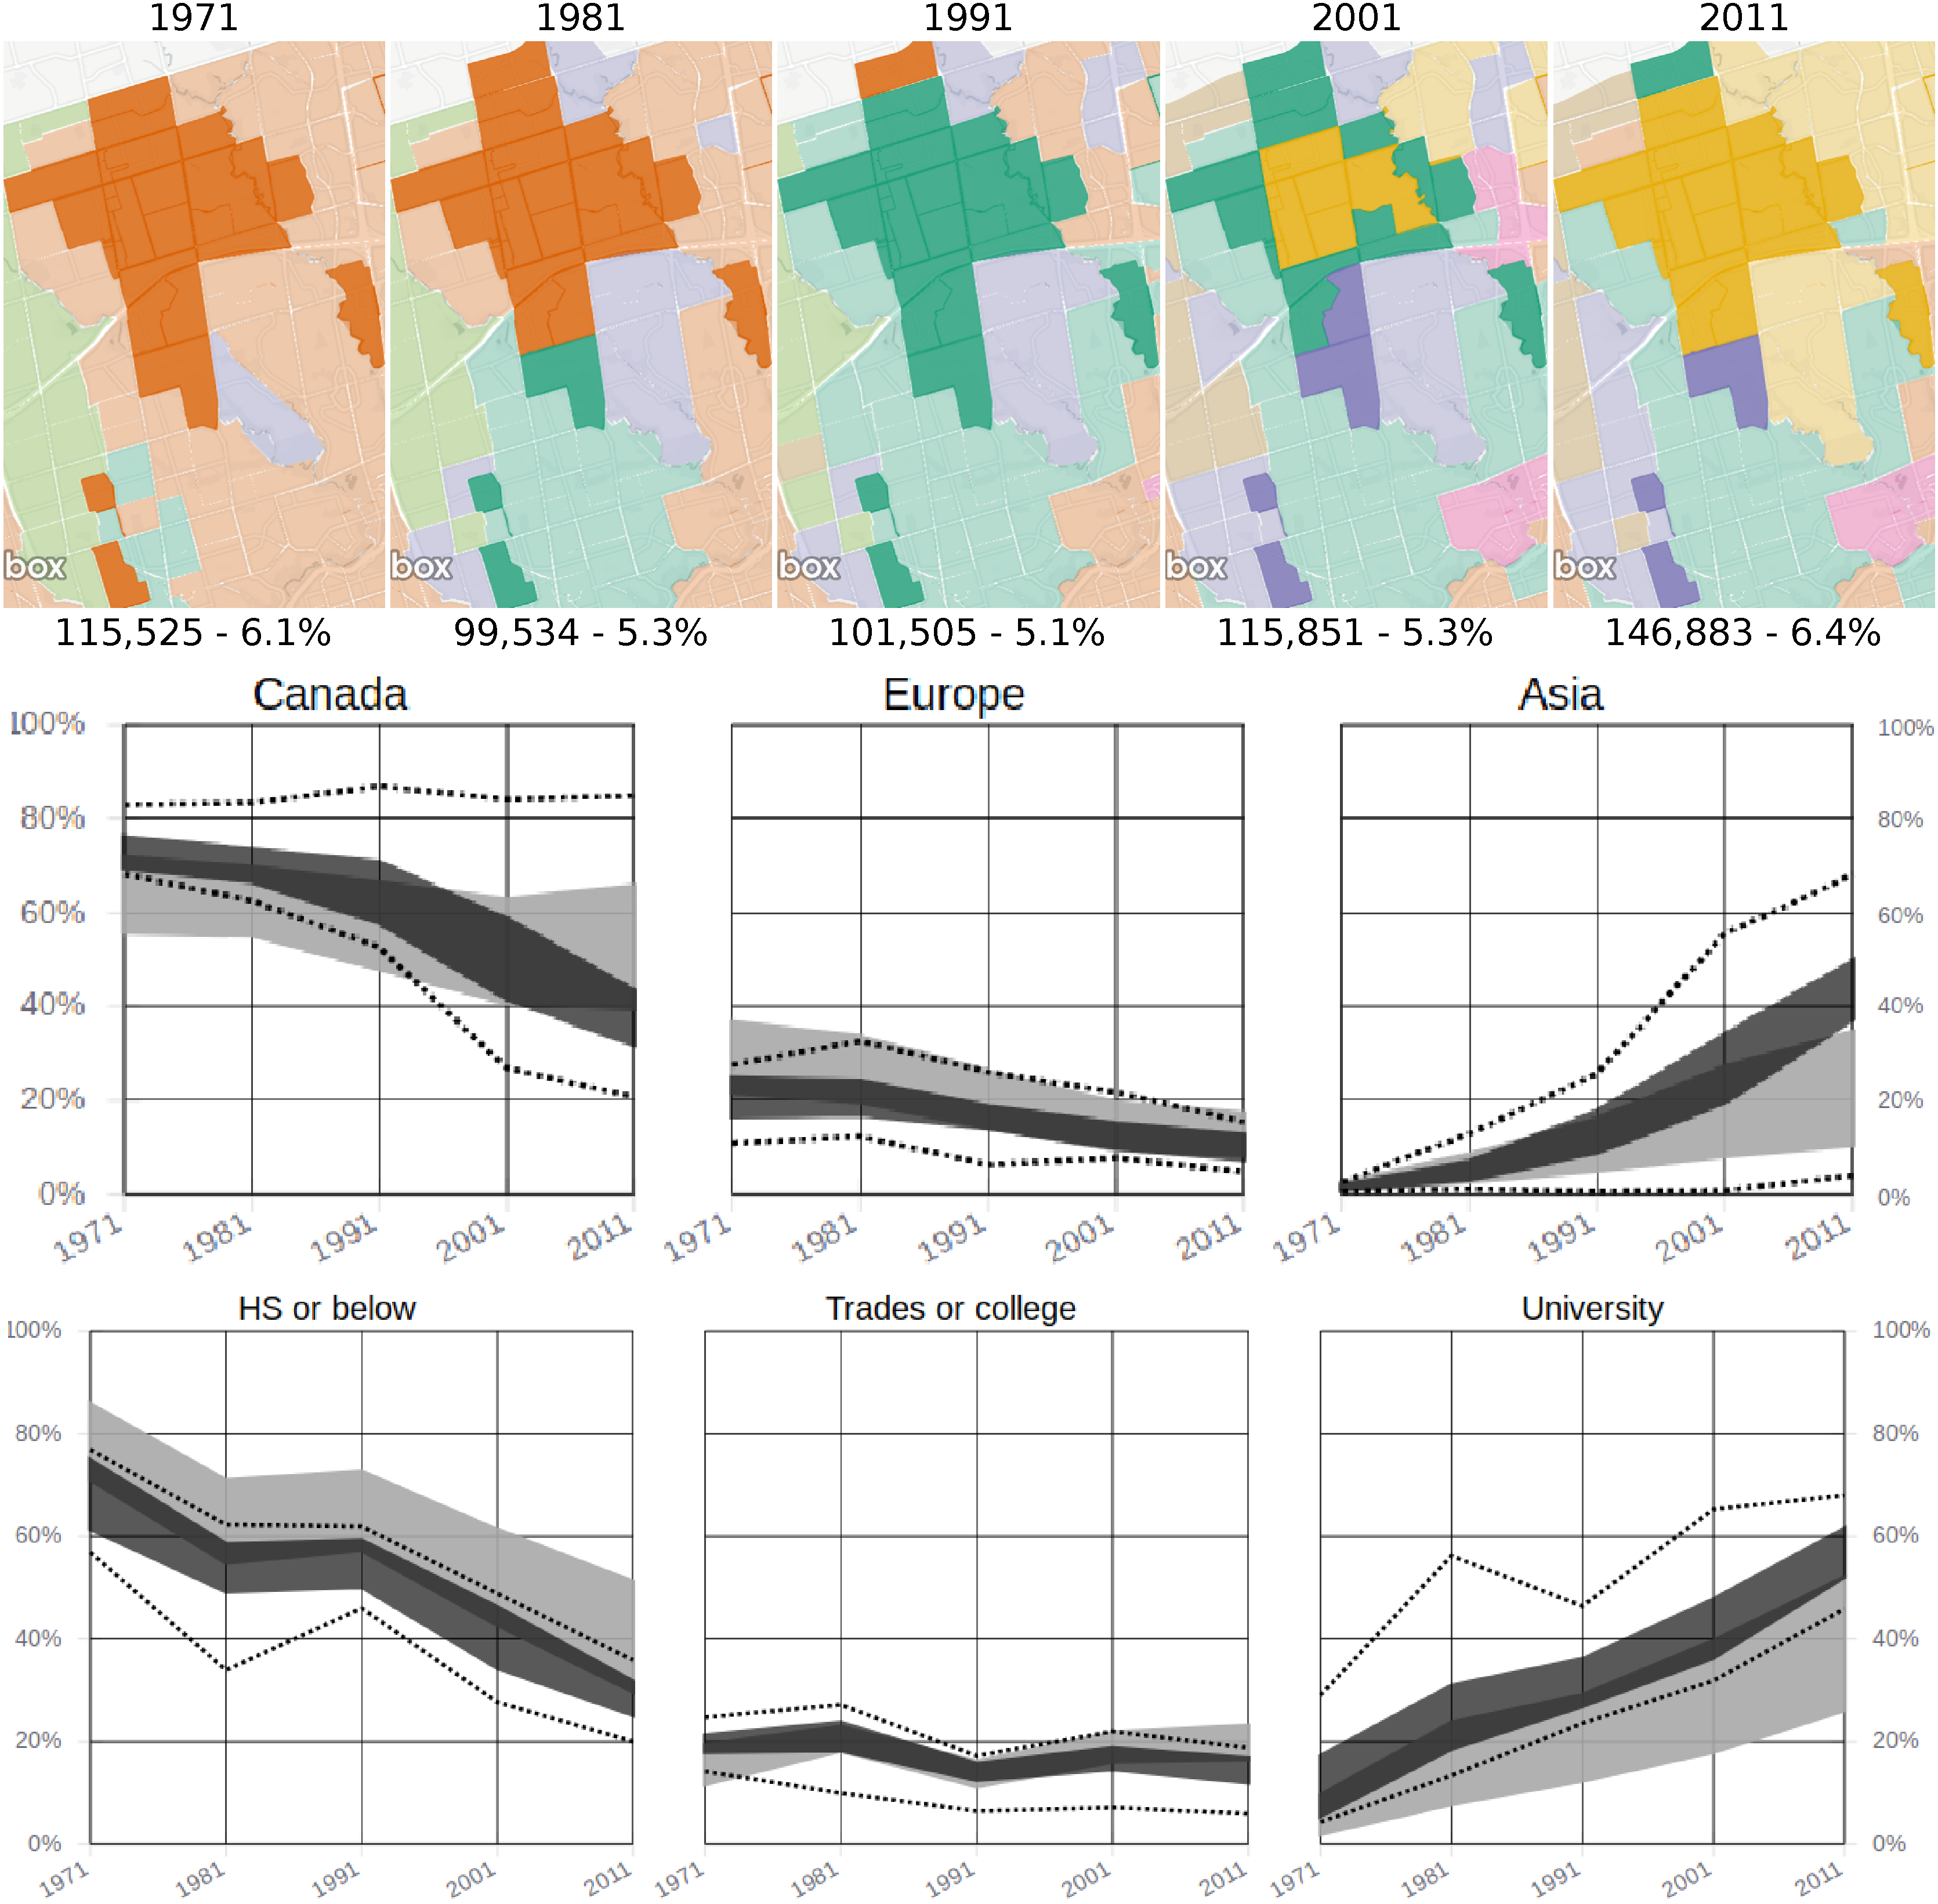
\includegraphics[width=0.75\linewidth]{toVol.pdf}
    \caption{Details for some regions of Toronto that were classified into 3 or
         more clusters over time.\label{fig:toVol}}
\end{figure}

In 2001, the purple cluster of high income annexes neighbouring parts of the
volatile region, and the Asian born population increases sharply, as illustrated
by the appearance of the yellow cluster.  This cluster indicates well educated,
higher income, and about 30\%-50\% Asian born population. By 2011, the yellow
cluster increased considerably, annexing parts of the high income purple
cluster, including the neighbouring Bridle Path area.

The geographical borders of the clusters obtained using our method are similar
to the regions presented by previous studies considering
Toronto~\citep{hulchanski2007three}. However, our interface provides a deeper
insight into their demographic composition, since we consider more data than
solely Average Income, which appears to be a good proxy variable nonetheless.
This scenario showcases the ability of our method and interface to capture and
understand the sources of urban volatility.

\section{Expert feedback}
\label{sec:expert}
As our method and tool are novel to the field, and somewhat exotic,  we
subjected them to the critical scrutiny of experts. We contacted academic and
industry experts in sociology and urban sciences to solicit their evaluation of
our methodology. They had access to the prototype tool, a descriptive
documentation of the features (included in the supplementary material), and a
sequence of documentation videos illustrating how to perform specific tasks. The
documentation explains which datasets are used and how the data is represented
and processed, noting explicitly that there is no geographic harmonisation. We
focused our inquires on the results obtained, asking if they found anything
interesting in the data. The message sent and their full response is included in
the supplementary material. Each of the five experts is identified by a letter,
from A to E. 



The overall overall response of the experts was positive,  mentioning that the
prototype allows them to analyse census data without the additional work of
obtaining and cleaning the data (A, B, E), and it allows the inclusion of
geographic visual analysis tools in their research process (D). It enables the
users to tell different stories about neighbourhoods/cities and their changes
(A), visualise the relationship between key urban variables over time (D),
offering a quick way to identify particular neighbourhoods that one may be
interested in studying more in depth around a particular issue or efficiently
understanding the context of an area (E).  Indeed, the experts identified
gentrification processes in Manhattan (B) and Dallas (E), reinforced a
hypothesis for occupational clustering (D), and highlighted how the method can
be used to compare neighbourhoods and cities (A). In summary, their view was that
the proposed methodology can be a viable alternative for the visual analytics of
evolving demographic data.



The interface was "easy to navigate" (B), but it was also considered
"overwhelming" (A), "intimidating" (E), and "tricky to interpret" (C), possible
side-effects of our effort to increase  representational accuracy, where we
avoided using simplified representation or labels. Identifying clusters by their
most relevant variables was welcome, but the overlap of information from
different clusters in the boxplot was "a bit confusing" (C) when colour was not
present. Further, most clusters can be sufficiently characterised using only the
most relevant aspect, but this is not generally true. 


While the map of trajectories was mentioned as a "good summary map", how it
related to the clustering method was unclear (C). The methods include different
options on how the colours are used, but both are works in progress since reliably
representing several distinct entities using colours is humanly unfeasible.
Indeed, the number of distinguishable colours was a significant constraint, we
found indications that more clusters should be used in some cases, even if eight
clusters is more than what is traditionally considered in these analyses.
Conversely, increasing the number of clusters would also complicate the
interpretation of the results.


The experts also mentioned the poor responsiveness of the method when changes in
the clustering parameters required server-side processing (B,D). Indeed, the
current implementation can take a few minutes to cluster regions with high
number of CTs, like Los Angeles or Brooklyn. Server-side processing reduced the
amount of data transferred to client, but it might increase the response time
under load. We implemented a caching policy, but fully pre-processing the
results is not practical due to size of the parameter space.

Most of the experts demonstrated interest in using our method in their research
(A, B, D, E), aiming to use the census data as a backdrop for other datasets,
providing demographic context. They also mentioned the need to export subsets of
data, plots, and maps to be used in reports and publications (C, D, E). More
importantly, while these experts were aware that our method does not perform
geographic harmonisation, none of them mention it. We did not specifically ask
if this difference led to unexpected results, but rather if they found
interesting insights. 

\section{Discussion and limitations}

The objective of this work was to leverage a graph based data representation
with visual tools to allow for the exploration of geographically inconsistent
census data. While we successfully replicated and corroborated results from the
literature, this method still has significant limitations. 

Removing the geographical normalization/interpolation step greatly reduces the
amount of work necessary, but the method still requires consistent variables
across the years. Matching the fields of the public census can be trivial for
some aspects, like Age, but challenging for others, like Income. The divulged
income ranges vary over time, the actual value changes due to inflation and
other factors, and so on. Moreover, some fields were not considered in earlier
censuses, such as Race in Canada, or Hispanic population in the USA, hampering its
use when they are available. We matched some aspects, but a deeper demographic
analysis would greatly benefit from all available information.


Another limitation is the lack of control on how much the geographical
information will impact the clustering result. While the adopted method met our
needs for this work, a configurable control would add another dimension to the
exploration, allowing for more intra-cluster variance to obtain more 'compact'
clusters. We explored changing the number of content based augmented edges, but
this proved to be unreliable and hard to interpret. The~\emph{ClustGeo}
method~\cite{Chavent2017} can be a viable option for this, allowing a graph
based input and a hierarchical output, combined using a single mixing
parameter. Alternatively, one could cluster the changes~\cite{bian2018survey}
instead of the stable states.


There are also technological limitations, such as memory use on the
visualization client. To allow for changes on the CTs over the years, we use a
geographic file that contains all possible intersections, which can grow rather
large if the original city was expansive and contained several CTs, like NYC or
LA. However, the most significant technological limitation relates to parameters
that are not immediately interactive, such as the clustering configuration.
Since the clustering is computationally expensive and performed on the server,
which allows for cached results, some changes can take a few minutes to be
considered, removing any possibility of a continuous exploration. 


Indeed, the cognitive load on the user is already significant, as we compromised
simplicity for accuracy. While other works labelled the clusters, as 'young
urban', 'struggling', and so on~\cite{Delmelle2016,Delmelle2017}, we show the
statistical characteristics of the clusters, which are harder to interpret, as
the data may have subtle nuances that labels would otherwise hide. This also led
to a crowded interface, mitigated somewhat the use of pop-up panels and collapsible
sections. For some cities, especially if they are small and stable, the panels
can appear redundant, but each provide a different way to interact with the
information that can ease the exploration process for larger and dynamic cities.


\section{Conclusion}
Our objective was to allow for the exploration of census data without
geographical harmonization, an original alternative to a challenging and
error-prone process. Our method was able to corroborate previous findings from
the specialized literature, with an increased level of detail due to our data
representation and visualization choices. The feedback from experts was positive
and most of them were able to extract insight from the prototype and
demonstrated interest in using it on their research efforts. Indeed, the experts
also demonstrated further interest in similar tools, indicating that visual
analytics methods can be valuable in this field. 



% if have a single appendix:
%\appendix[Proof of the Zonklar Equations]
% or
%\appendix  % for no appendix heading
% do not use \section anymore after \appendix, only \section*
% is possibly needed

% use appendices with more than one appendix
% then use \section to start each appendix
% you must declare a \section before using any
% \subsection or using \label (\appendices by itself
% starts a section numbered zero.)
%


% \appendices
% \section{Proof of the First Zonklar Equation}
% Appendix one text goes here.

% % you can choose not to have a title for an appendix
% % if you want by leaving the argument blank
% \section{}
% Appendix two text goes here.


% use section* for acknowledgment
\ifCLASSOPTIONcompsoc
  % The Computer Society usually uses the plural form
  \section*{Acknowledgements}
\else
  % regular IEEE prefers the singular form
  \section*{Acknowledgement}
\fi


This research was supported by a University of Toronto Connaught Global
Challenge grant and is part of the Urban Genome Project. The authors thank Cary
Wu, Ethan A. Fosse, Fernando Calderón Figueroa, Patrick Adler, and James Murdoch
for their expert opinions; Mark S. Fox, Robert M. Wright, Ultan Byrne, Matti
Siemiatycki, Shauna Brail, and Richard Florida for general guidance and support;
and the anonymous reviewers for their constructive comments.



% Can use something like this to put references on a page
% by themselves when using endfloat and the captionsoff option.
\ifCLASSOPTIONcaptionsoff
  \newpage
\fi



% trigger a \newpage just before the given reference
% number - used to balance the columns on the last page
% adjust value as needed - may need to be readjusted if
% the document is modified later
%\IEEEtriggeratref{8}
% The "triggered" command can be changed if desired:
%\IEEEtriggercmd{\enlargethispage{-5in}}

% references section

% can use a bibliography generated by BibTeX as a .bbl file
% BibTeX documentation can be easily obtained at:
% http://mirror.ctan.org/biblio/bibtex/contrib/doc/
% The IEEEtran BibTeX style support page is at:
% http://www.michaelshell.org/tex/ieeetran/bibtex/
\bibliographystyle{IEEEtran}
% argument is your BibTeX string definitions and bibliography database(s)
\bibliography{IEEEabrv,rev}
%

% biography section
% 
% If you have an EPS/PDF photo (graphicx package needed) extra braces are
% needed around the contents of the optional argument to biography to prevent
% the LaTeX parser from getting confused when it sees the complicated
% \includegraphics command within an optional argument. (You could create
% your own custom macro containing the \includegraphics command to make things
% simpler here.)
%\begin{IEEEbiography}[{\includegraphics[width=1in,height=1.25in,clip,keepaspectratio]{mshell}}]{Michael Shell}
% or if you just want to reserve a space for a photo:

% \begin{IEEEbiography}{Fabio Dias}
% Biography text here.
% \end{IEEEbiography}

% % if you will not have a photo at all:
% \begin{IEEEbiographynophoto}{Daniel Silver}
% Biography text here.
% \end{IEEEbiographynophoto}

% insert where needed to balance the two columns on the last page with
% biographies
%\newpage

% You can push biographies down or up by placing
% a \vfill before or after them. The appropriate
% use of \vfill depends on what kind of text is
% on the last page and whether or not the columns
% are being equalized.

%\vfill

% Can be used to pull up biographies so that the bottom of the last one
% is flush with the other column.
%\enlargethispage{-5in}



% that's all folks
\end{document}


